%# -*- coding: utf-8-unix -*-
% !TeX spellcheck = zh_CN
\documentclass[oneside,UTF8,a4paper,12pt]{book}		% twoside 表示双面打印

\usepackage{url}
\usepackage{cite}
\usepackage{color}
\usepackage{xcolor}
\usepackage{import}
\usepackage{fancyhdr}
\usepackage{hyperref}								% 添加超链接
\usepackage{graphicx}
\usepackage{enumitem}
\usepackage{listings}								% 代码
\usepackage{transparent}
\usepackage{indentfirst}							% 段首缩进
\usepackage{supertabular}							% 长表格(换页处理)
\usepackage[utf8]{inputenc}
\usepackage[center]{titlesec}						% chapter1修改为第1章

\graphicspath{{./img/}}

\setlength{\parindent}{2em}							% 段首缩进
\setlength{\parskip}{.5em}							% 段落间距
\renewcommand{\baselinestretch}{1.3}				% 行间距

% 页眉
\pagestyle{fancy}
\renewcommand{\chaptermark}[1]{%
	\markboth{第\,\thechapter\,章\ #1}{}}

% 自定义命令

% 章节汉化
\titleformat{\chapter}{\raggedright\Huge\bfseries}{第\,\thechapter\,章}{1em}{}
\titleformat{\section}{\raggedright\Large\bfseries}{\,\thesection\,}{1em}{}
\titleformat{\subsection}{\raggedright\large\bfseries}{\,\thesubsection\,}{1em}{}
\titleformat{\subsubsection}{\raggedright\normalsize\bfseries}{\,\thesubsection\,}{1em}{}

% 目录居中
\renewcommand*\contentsname{\hfill 目录 \hfill}

% 设置itemize行间距
\setitemize{
	itemsep=0pt,
	partopsep=0pt,
	parsep=0.8em,
	topsep=5pt}
	
% 代码颜色设置
\definecolor{codegreen}{rgb}{0,0.6,0}
\definecolor{codegray}{rgb}{0.5,0.5,0.5}
\definecolor{codepurple}{rgb}{0.58,0,0.82}
\definecolor{backcolour}{rgb}{0.95,0.95,0.92}

\lstdefinestyle{mystyle}{
	backgroundcolor=\color{backcolour},   
	commentstyle=\color{codegreen},
	keywordstyle=\color{magenta},
	numberstyle=\tiny\color{codegray},
	stringstyle=\color{codepurple},
	basicstyle=\ttfamily\footnotesize,
	breakatwhitespace=false,         
	breaklines=true,                 
	captionpos=b,                    
	keepspaces=true,                 
	numbers=left,                    
	numbersep=5pt,                  
	showspaces=false,                
	showstringspaces=false,
	showtabs=false,                  
	tabsize=2
}
\lstset{style=mystyle}

% 定义
\newtheorem{note}{注意:}

% 去掉超链接红框
\hypersetup{hidelinks,
	colorlinks=true,
	allcolors=blue,
	pdfstartview=Fit,
	breaklinks=true}

\makeatletter
\def\UrlAlphabet{%
	\do\a\do\b\do\c\do\d\do\e\do\f\do\g\do\h\do\i\do\j%
	\do\k\do\l\do\m\do\n\do\o\do\p\do\q\do\r\do\s\do\t%
	\do\u\do\v\do\w\do\x\do\y\do\z\do\A\do\B\do\C\do\D%
	\do\E\do\F\do\G\do\H\do\I\do\J\do\K\do\L\do\M\do\N%
	\do\O\do\P\do\Q\do\R\do\S\do\T\do\U\do\V\do\W\do\X%
	\do\Y\do\Z}
\def\UrlDigits{\do\1\do\2\do\3\do\4\do\5\do\6\do\7\do\8\do\9\do\0}
\g@addto@macro{\UrlBreaks}{\UrlOrds}
\g@addto@macro{\UrlBreaks}{\UrlAlphabet}
\g@addto@macro{\UrlBreaks}{\UrlDigits}
\makeatother

% 字体
\usepackage{xeCJK}
\usepackage{graphicx}
\usepackage{fontspec} 
\setCJKmainfont{Source Han Mono SC} 


\begin{document}

\author{丁敬}
\title{X 教程}
\date{2023年04月26日}

\frontmatter										% 对前言和概览用罗马数字作为页码
\mainmatter      		 							% 对正文用阿拉伯数字作为页码
\maketitle
\tableofcontents									% 目录


\mainmatter
\begin{sloppypar}									% 自动换行
\chapter{新手开发者指南}

\section{X系统概念}

本章旨在向您介绍您需要了解的X窗口系统的基本概念和术语。当你有了这些概念,你将准备在后面的章节中更深入地研究特定的主题。

\subsection{X基于C/S结构}

X被设计成允许多个程序共享对一组公共硬件的访问。这种硬件既包括输入设备,如鼠标和键盘,也包括输出设备,如视频适配器和连接到它们的显示器。这些公共硬件由指定的某个进程进行统一管理,这个进程称为X服务端(因为它向客户机应用程序提供硬件设备的服务)。


与许多C/S系统一样,X服务端通常向许多同时运行的客户机提供服务,因此X服务端比大多数客户机运行的时间更长,并侦听来自新客户机的传入连接。


许多用户只在独立的笔记本电脑或桌面系统上使用X。在此设置中,X客户端与X服务器运行在同一台计算机上。然而,X为客户端/服务器通信定义了一个流协议。该协议可以通过网络公开,以允许客户端连接到不同机器上的服务器。这里需要注意的是,在这个模型中,客户机/服务器标签可能会令人困惑。此时在你面前的笔记本如果显示了远程机器客户端生成的图形,那么你当前的笔记本就是X服务端,生成图形的远程机器则是X客户端,如图 \ref{img-1.1.1-1}。


\begin{figure}[h]
    \centering
    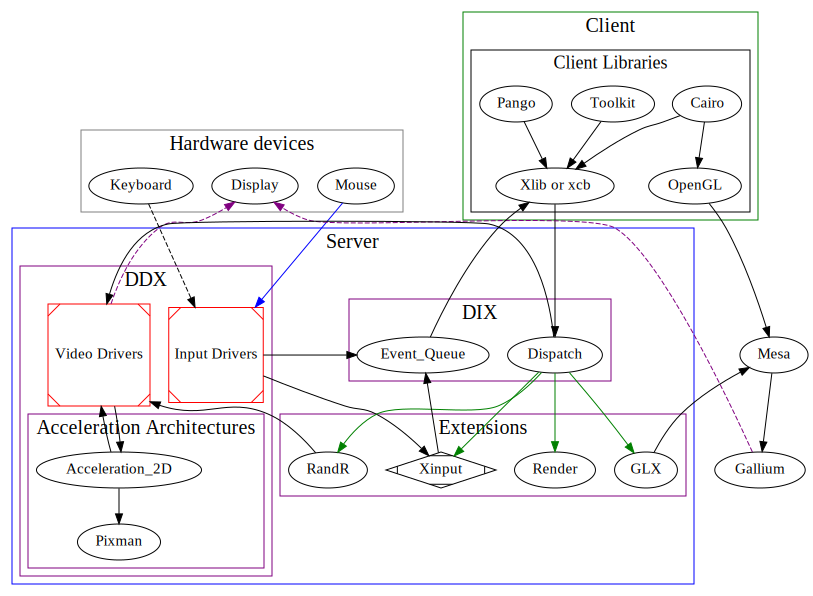
\includegraphics[scale=0.40]{x-1-1.png}
    \caption{X客户端/服务端模型}
    \label{img-1.1.1-1}
\end{figure}

\subsection{X实践}

本节描述X的一些基本组件及其工作原理。这个部分内容很多,有点像大杂烩。推荐的阅读方法是浏览一遍,然后回过头再读一遍。

\subsubsection{通过键盘输入}

X服务执行的任务之一是处理键盘上的输入,并将相应的键事件发送到适当的客户机应用程序。在简单的X配置中,每次只有一个客户端具有“输入焦点”,并且大多数关键事件将发送到该客户端。根据窗口管理器配置,只需将鼠标移动到另一个窗口、单击鼠标、使用热键或操作显示可用客户机的面板,就可以将焦点移动到另一个窗口。具有焦点的客户端通常以某种方式突出显示,以便用户可以知道他们的输入将流向何处。客户端可以使用“抓取”(在本章后面描述)来覆盖向重点客户端发送关键事件的默认交付。

世界上有各种各样的键盘。这是由于不同的语言要求,不同的国家标准,以及硬件供应商试图区分他们的产品导致的。这种多样性使得从硬件的“键码”到文本输入的按键映射成为一个具有挑战性和复杂的过程。X服务在按键按下和释放事件中报告一个简单的8位键值代码。X服务还提供从这些键码到“KeySyms”的键盘映射,“KeySyms”表示键上的符号标签(“a”、“Enter”、“Shift”等)。在给定的会话之外,键码没有固有的意义;相同的键可能在不同的键盘、服务器、配置或操作系统上生成不同的代码值。KeySym值是全局分配的常量,因此是大多数应用程序应该关注的。X Keyboard (XKB)扩展提供了复杂的配置和布局处理,以及原始协议中缺少的额外键码处理功能。Xlib和工具包还为更高级的输入函数提供了输入方法,例如组合键处理或将键序列映射到复杂字符(例如,亚洲语言输入)。

\subsubsection{通过鼠标输入}

X协议定义了一个输入“指针”。指针在屏幕上由光标表示;它通常由鼠标或类似的输入设备控制。应用程序可以控制光标图像。核心协议包含简单的2色光标图像支持。渲染扩展提供了alpha混合32位颜色光标支持;这种支持通常通过libXcursor访问。

指针设备报告运动事件、按钮按下、按钮释放事件给客户端。Xorg服务的默认配置只有一个指针。这个指针聚合了连接到服务器的所有指针类型设备的运动和按钮事件:例如,笔记本电脑的触摸板和外部USB鼠标。用户可以使用Xinput扩展2.0中的MultiPointer X (MPX)功能来启用多个游标,并为每个游标分配设备。使用MPX,每个指针都有自己的输入焦点。每个指针都与键盘配对,键盘向具有该指针输入焦点的客户机提供输入。

\subsubsection{通过触摸板输入}

对于基本输入,触摸板对客户来说只是移动指针和生成按钮事件的另一个设备。可以使用Xinput扩展2.2版本(随Xorg 1.12一起发布)或更高版本来支持多点触摸事件报告。

\subsubsection{通过触摸屏输入}


\subsubsection{高级输入设备和技术}


\subsubsection{从显示器读取图像}

X服务不跟踪它在显示器上绘制的内容。一旦图片二进制流被呈现到帧缓冲区,X服务对它们的责任就结束了。如果需要重新渲染图片(例如,因为它们暂时被遮蔽了),X服务器会请求客户端(通常是合成管理器或最初绘制它们的应用程序)重新绘制它们。

在某些情况下,特别是在截屏时,客户端需要直接读取帧缓冲区的内容。X协议为这种情况提供了一个GetImage请求。

GetImage有许多缺点,除非绝对必要,否则应该避免使用。GetImage通常非常慢,因为现代图形硬件为输出彩色图像而优化的,而代价是需要耗费算力渲染图像中的每个像素。在这里,底层硬件把请求的帧缓冲区内容与帧缓冲区的对齐、填充和字节排序一起呈现给客户端。Xlib和XCB中提供了相关代码,用于将帧缓存区的内容转换为对客户端有用内容,但是,这个过程非常复制,因此此代码效率很低。

\subsection{输出}

\subsubsection{渲染/栅格化}

X协议最初定义了一组核心的基本渲染(注:渲染有时候也称栅格化\footnote{栅格化:又称光栅化,是将向量图形格式的图像转换为点阵图以用于显示器或打印机输出的过程。})操作,如线条绘制、多边形填充和图像缓冲区的复制。它们并没有随着现代应用程序所期望的图形硬件和操作的发展而发展,因此现在主要用于遗留应用程序。

现代应用程序使用各种客户端渲染库,例如用于渲染2D图像的Cairo或用于3D渲染的OpenGL。然后这些可以将图像推送到X服务进行显示,或者使用DRI绕过X服务器并直接与本地视频硬件交互,利用GPU加速和其他硬件功能。


\subsubsection{多边形渲染模型}


\subsubsection{显示器和屏幕}

X将机器的资源划分为显示器和屏幕。显示器通常是连接到单个X服务的所有设备,并为单个用户显示单个会话。系统可以有多个显示器,例如多座位设置,或者甚至在系统控制台上有多个虚拟终端。每个显示器都有一组输入设备,以及一个或多个与之相关联的屏幕。屏幕是显示的一个子集,窗口可以在屏幕上显示或移动,但是窗口不能跨多个屏幕或从一个屏幕移动到另一个屏幕。输入设备可以与X服务器所有屏幕上的窗口交互,例如将鼠标光标从一个屏幕移动到另一个屏幕。最初,每个屏幕都是一个带有单个显示器的显示适配器,但现代技术允许将多个设备组合成逻辑屏幕或将单个设备分开。

在将客户机连接到X服务器时,必须通过\lstinline|$DISPLAY|环境变量或者应用程序选项指定要连接到哪个显示器,如:\lstinline|-display|或\lstinline|--display|等。完整的DISPLAY语法记录在X(7)手册页中,但是完整的显示语法是\lstinline|hostname: DISPLAY.screen|。对于本地连接,\lstinline|hostname|可以省略,\lstinline|.screen|也可以省略,只留下\lstinline|:display|,例如:\lstinline|:0|以表示使用X服务默认的显示屏幕。

\subsubsection{图形上下文(GC)}

图形上下文(GC)是一种结构,用于存储X绘图操作的共享状态和公共值,以避免每次请求都必须重新发送相同的参数。客户端可以根据需要分配额外的图形上下文,以便能够通过为每组值设置单独的GC,然后为每个操作指定适当的GC来指定不同的值。


\subsubsection{颜色和视觉效果}

X太老了,当它被设计出来的时候,大多数用户使用的是单色显示器,只有黑白像素可供选择,即使在那时,硬件制造商就0和1分别代表黑白或白黑也无法达成一致。那些多花了1000美元的人将拥有4位或8位颜色,允许从多达256种颜色的调色板中选择像素。但现在是2012年了,每个像素没有32位色彩数据的人都是勒德分子。尽管如此,这里仍然存在很多复杂性,需要有人来解释……

\subsubsection{同步和刷新}

正如在通信一章中所描述的,X协议试图通过尽可能多地执行异步操作来避免延迟。新程序员特别注意到这一点,他们调用渲染函数,然后想知道为什么既没有返回错误也没有看到预期的输出出现。由于绘图操作不需要等待来自X服务器的响应,因此它们只是被放置在客户机的传出请求缓冲区中,而不是发送到X服务,直到某些事情导致缓冲区被刷新。缓冲区被填满后将自动刷新,但是在Xlib中需要很多命令来填充默认的32kb缓冲区大小。当调用阻塞等待服务器响应的函数时,Xlib和XCB将刷新缓冲区(尽管由于设计模型不同,两者之间的函数有所不同—详细信息请参阅Xlib和XCB章节)。最后,客户端可以专门调用Xlib中的\lstinline|XFlush()|或XCB中的\lstinline|xcb_flush()|,将所有排队的请求从缓冲区发送到服务器。为了刷新缓冲区并等待X服务器完成对缓冲区中所有请求的处理,客户机可以调用Xlib中的\lstinline|XSync()|或XCB中的\lstinline|xcb_aux_sync()|。

\subsection{X窗口系统中的对象}

X中使用到的各种各样的对象。


\subsubsection{窗口(Windows)}

在X中,窗口只是屏幕的一个区域,可以在其中进行绘图。窗口被放置在树形层次结构中,根窗口是服务器创建的窗口,它覆盖整个屏幕表面,并在服务器的生命周期内存在。所有其他窗口都是根窗口的子窗口。大多数用户认为窗口的UI元素只是窗口层次结构的一个层次。

在层次结构的每一层,窗口都有一个堆叠顺序,控制当兄弟窗口相互重叠时可以看到窗口的哪些部分。客户端可以注册可见性通知信号,以便在窗口变得比以前更可见或更不可见时获得事件,X客户端通过这一信号来优化仅绘制窗口的可见部分。

在传统X环境中因为X服务不知道客户端窗口的内容,所以当客户端窗口的一部分被覆盖并且需要绘制时,运行的客户机也会收到expose事件。当窗口管理器处于活动状态时,客户端通常不会接收到expose事件,因为窗口管理器将每个窗口的内容放在单独的、不重叠的屏幕外缓冲区中,然后将每个窗口的可见段组合在屏幕上显示。由于客户端无法确认其是运行在传统X环境中还是含有窗口管理器的环境中,因此客户端必须处理好expose事件。

\subsubsection{像素图(Pixmaps)}

像窗口一样,像素图是可以进行绘图的区域。与窗口不同,像素图不是层次结构的一部分,也不直接显示在屏幕上。像素图的内容可以复制到窗口显示,或者直接通过请求,如CopyArea,或自动设置窗口的背景为给定的像素图。像素图可以存储在系统内存、图形适配器上的视频内存、客户端和服务器都可以访问的共享内存中。给定的像素图可以根据需要在系统和视频内存之间来回移动,以便在更快的访问视频RAM中维护最近访问的像素图的良好缓存。使用MIT-SHM扩展在共享内存中存储像素图可以允许客户端更快地推送更新,因为它直接在共享内存区域上操作,而不必通过套接字将数据复制到服务器,但它也可能阻止服务器将像素图移动到视频ram中的缓存中,从而使复制到屏幕上的窗口变慢。

\subsubsection{小部件(Widgets)}

应用程序需要的不仅仅是窗口和像素图来提供用户界面——用户希望在他们的窗口中看到菜单、按钮、文本字段、菜单等。这些用户界面元素在大多数环境中统称为小部件(widget)。X实际上并没有在核心协议或库中提供任何小部件,只提供了诸如呈现方法和输入事件之类的构建块。像Qt和GTK+这样的工具包为应用程序提供了一组通用的小部件,并提供了一组丰富的功能,为广泛的用途和用户提供了良好的支持。

\subsubsection{XIDs}

服务器管理的许多资源都从服务器范围的名称空间分配了一个称为XID的32位标识号。每个客户端在第一次连接到X服务器时被分配一个标识符范围,每当它发送一个请求来创建一个新的Window、Pixmap、Cursor或其他XID标记的资源时,客户端(通常在Xlib或xcb库中透明地)从它的范围中选择一个未使用的XID,并将其包含在向服务器发出的请求中,以标识由该请求创建的对象。这允许将对新资源进行操作的进一步请求发送到服务器,而不必等待服务器处理创建请求并返回标识符分配。由于名称空间对于Xserver是全局的,因此客户机可以在某些上下文中从其他客户机引用XID,例如移动属于另一个客户机的窗口。

\subsubsection{Atoms}

为了减少X协议中常见字符串的重传,使用了一个简单的查找表机制。该表中的条目被称为Atoms,它们有一个整数键(在大多数需要它们的协议操作中传递)和一个文本字符串(可以根据需要检索)。interatom操作查找给定字符串的Atom id号,并且可以选择将该字符串添加到表中,如果还没有找到,则返回一个新id。GetAtomName返回给定Atom id号的字符串。Atoms 用于各种各样的请求和事件,但是在给定X服务器的所有操作和客户端中具有唯一的名称空间。

\subsubsection{属性(Properties)}

X中用于提供可扩展元数据的常见设计模式是Property机制。Properties是一个键值对,其中键是一个文本字符串,表示为X Atoms,值是一个类型化的值,也可以是一个Atoms、整数或其他类型。核心协议提供了窗口(Window)和字体(font)的Properties。Xinput扩展向输入设备添加Properties,Xrandr扩展向输出设备添加Properties。

X本身不赋予窗口属性任何意义或目的。但是,已经为许多窗口属性建立了约定,以提供对窗口和会话管理有用的元数据。初始属性集在X客户机间通信约定手册(ICCCM)中定义,该手册可在 \url{http://www.x.org/releases/current/doc/}上找到。这个最初的集合后来被致力于现代桌面环境通用功能的小组在freedesktop.org上进行了扩展,它成为了扩展窗口管理器提示(extended Window Manager Hints, EWMH)规范,可以在 \url{http://www.freedesktop.org/wiki/Specifications/wm-spec}上找到。

\subsubsection{抓取(Grabs)}

X中的Grabs提供了锁定和保留功能。“激活Grabs”立即独占控制给定资源,并锁定所有其他客户端,直到Grabs被释放。“被动Grabs”在资源上放置了一个预留,导致在稍后发生事件(比如:按键)时触发主动抓取。例如,无论当前哪个应用程序具有输入焦点,都可以使用热键转到某个应用程序。

其中一个可用的Grabs是服务器抓取。抓取服务器的客户端会锁定所有其他客户端,从而阻止任何其他应用程序更新显示或与用户交互,直到服务器Grabs被释放。这应该尽快发布,因为它除了在用户无法切换到其他程序时惹恼用户外,还可能导致安全问题,因为屏幕锁只是另一个客户端,将与其他客户端一起被锁定。

Grabs的另一种主要形式是在输入设备或事件上。客户端可以主动抓取键盘或鼠标来强制从设备获取所有输入,即使光标移动到应用程序窗口之外。被动抓取可以放置在特定的输入事件上,例如特定的按键事件或鼠标按钮事件,从而在事件发生时自动为该客户端发生主抓取。

更多信息查看:
\url{http://who-t.blogspot.com/2010/11/high-level-overview-of-grabs.html}

\section{X客户端与X服务端通信}

X客户端库和服务器处理了编码、解码和传输X协议的大部分细节。然而,为了能够开发和调试X客户机、服务器代码和驱动程序代码,通常需要对通信模型有一个基本的了解。

X客户机和服务器之间的通信通道是全双工的:任何一方都可以在任何时间向另一方发送消息。这通常是通过TCP/IP套接字接口实现的,但也经常使用其他通信通道,包括Unix域套接字、命名管道和共享内存。通道必须提供可靠的、有序的字节流——X协议没有提供重新排序或重新发送数据包的机制。例如,对于TCP/IP连接,使用TCP而不是UDP。

通过X通信通道发送的消息由X协议(Version 11:简称X11)定义。该议定书最初发表于1987年。虽然在过去的25年里它已经得到了极大的扩展,但核心协议仍然与原始定义兼容。协议规范文档可以在\url{http://www.x.org/releases/current/doc/}上阅读。

X11协议的关键特性之一是它的扩展机制。虽然核心协议在过去几年中发生了一些小的向后兼容变化,但大多数演变都是通过对协议的可选扩展进行的。核心协议提供了一种机制来列出和查询X服务器支持的扩展,并将这些扩展的消息添加到客户端和服务器之间的通信中所支持的集合中。服务器构建者可以选择支持哪些扩展,开发人员可以随着用例的发展添加或删除扩展,而不必担心破坏与核心协议的兼容性。客户端需要检查他们需要的扩展。如果扩展不存在(在适当的版本级别),客户端可能会退回到提供功能较差的接口,或者通知用户扩展丢失并失败。

当X客户端首次连接到X服务器时,会发生握手过程,以建立通道,验证客户端是否通过连接身份验证,并设置一些通信参数,例如要使用的字节序。在X的早期,人们认为服务器是一台功能强大的机器,而客户机不是。因此,有趣的是,客户机可以要求服务器提供客户机喜欢的任何端序:服务器将根据需要交换请求和响应的字节。

之后,客户端向X服务器发送请求消息,要求服务器执行操作或向客户端提供一些信息。客户端通常在缓冲区中积累请求,分批发送请求,以获得更有效的通信处理和上下文切换。该缓冲区通常由Xlib或XCB为客户端提供和管理;客户机应用程序经常需要将缓存的请求刷新到X服务器,以确保及时处理。

X服务器按照从每个客户机接收到的顺序处理来自该客户机的请求。但是,服务器通常在任何给定时间对来自多个客户机的请求进行多路复用,并且不保证客户机之间的任何排序,除非发出特殊请求以确保这一点。服务器和客户端都跟踪到目前为止在它们的连接上发送的请求的数量,并使用该数字作为每个请求的序列号,以便以后识别它。

服务器向客户端发送响应。来自客户机的许多请求仅由X服务器处理,如果一切正常,则不会返回任何内容给客户机。如果将请求定义为返回信息,则服务器将向客户机发送一个称为应答的响应。应答的序列号标识应答数据作为响应的请求。客户机可能一次向X服务器发送了许多请求,并且正在异步等待响应。应答将按顺序返回,但客户机需要记住请求序列号,以便将应答映射回所发出的请求。

如果在处理请求时出现问题,那么X服务器将向客户机发送一个错误响应。错误响应包括有问题的数据包的序列号、错误代码和有关出错原因的其他详细信息。调试故障通常涉及确定错误请求的来源。由于协议的异步性,错误响应通常在客户端转移到稍后的调用之后才被接收;因此,序列号在这里是无价的信息。

客户端还可以注册以获得来自X服务器的各种事件通知。事件发生时,作为特定的响应类型从服务器发送到感兴趣的客户端。事件可能由以下因素引起:


\begin{itemize}
	\item 用户输入,例如移动鼠标或在键盘上打字
	\item 另一个客户端,比如移动窗口的窗口管理器
	\item 外部事件,例如设备正在与系统连接或断开。
\end{itemize}

工具箱和X协议库具有检查是否从X服务器接收到任何事件的功能。大多数X应用程序都是由一个主“事件循环”驱动的,该循环捕获事件响应并适当地处理它们。

在X11协议中,每个请求和响应类型都有一个8位标识码,用于确定发出信号的是哪个操作、事件或错误。这些代码在每个通信方向上都是唯一的。例如,从客户机到服务器的任何以字节值3开头的消息都是\lstinline|getwindowatattributes|请求。错误和事件有单独的编号空间:错误代码3表示BadWindow错误,而事件代码3表示KeyRelease事件。

通信协议的许多特性都经过调整,以支持许多年前的计算环境。例如,请求序列号根本不由客户端传输:客户端和服务器大概可以保持计数。响应序列号仅部分传输,使用智能协议加上计数来跟踪其余部分。类似地,服务器上的资源在协议请求中使用称为XID的小整数标识。XID实际上是由客户机从服务器提供给它们的XID空间分配的。这两种优化,以及8位请求/响应ID空间,都是由于希望在网络上有非常小的数据包而产生的。这样,就可以在屏幕上用很少的字节沿一个方向移动来绘制一条线。

扩展可以根据需要向核心协议添加请求、事件和错误。X服务器在服务器启动时动态地为扩展消息分配代码。因此,相同的扩展在不同配置的服务器上可能具有不同的值。在当前运行的X服务器上使用的值可以通过命令\lstinline|xdpyinfo -queryExtensions|显示。只有256个8位数字,因此扩展通常会尝试保留这个空间:扩展将添加单个请求或事件代码,然后使用第二个字节作为“次要”代码来标识特定于该扩展的子消息。


\subsection{X协议安全模型}

核心X协议有一个相当简单的安全模型。在连接时检查客户端的地址,以查看是否允许连接到服务器:如果不允许,则拒绝连接。如果允许客户端连接,那么它将被授予对服务器的完全访问权限。这包括能够向所有客户端发送消息,监视所有设备的状态(包括所有击键、鼠标移动等)。客户端甚至可以请求X服务器终止另一个客户端的连接。

各种扩展都添加了细粒度的可选安全模型。“安全”扩展提供了一个简单的“可信”与“不可信”客户端的区别。SELinux和Solaris Xtsol扩展提供了更复杂的多级安全模型。

\subsection{身份验证方法}

X客户端被认证为允许连接到X服务器的机制随着时间的推移而发展。大多数服务器支持多种选择。

\subsubsection{xhost}

最初的连接安全方法是基于主机的身份验证,在这种方法中,给定主机上的任何用户或程序都被授予连接权限。默认情况下,只有本地主机可以连接,但是可以使用“xhost + hostname”来添加其他主机。这种机制有些幼稚:它假设每台机器只有一个用户,或者所有用户都同样值得信任。xhost机制在以后的版本中得到了扩展,以添加通过相同机制控制的其他访问控制方法。

这些方法包括一个可扩展的“服务器解释”方案,该方案只将字符串传递给X服务器,并允许X服务器根据需要定义新的访问控制类型。最常见的服务器解释方案是“localuser”,它使用现代操作系统中提供的接口来获取连接程序的用户id以进行身份验证。xhost和Xsecurity手册页提供了关于这个主题的更多细节。
	
\subsubsection{xauth}

目前最常用的身份验证方法是基于客户机和服务器之间的共享密钥。这是后来添加到X11协议的,它解决了xhost身份验证的许多问题。支持几种形式的秘密共享。最基本的是MIT-MAGIC-COOKIE-1。启动X服务器和会话(xinit、gdm、xdm等)的程序只是选择一个随机的128位数字,并将其记录在通过“-auth”命令行选项传递给X服务器的文件中,并将其记录在Xauthority文件中(在“\lstinline|$HOME/.Xauthority|”
或“\lstinline|$XAUTHORITY|”)。

如果客户端可以读取文件并向服务器提供正确的值,则允许连接。当使用SECURITY扩展时,cookie还可以将客户端标识为可信或不可信,并适当地授予权限。xauth和Xsecurity手册页提供了更多的详细信息。

\subsection{X服务器内的访问控制}

过去,应用程序在大小和复杂性上是有限的,而且相当可信。这种情况已经不再适用了,因为用户必须处理专有软件或大型软件,如web浏览器,这些软件可能是包含恶意代码(比如:缓冲区溢出利用)。不幸的是,一旦X客户端在X服务器上通过身份验证,它就可以通过以下几种方式与其他X客户端进行交互:

\begin{itemize}
	\item 重定向输入
	\item 屏幕截图/透明渲染
	\item 读写剪切板
	\item 修改其他X客户端的属性
\end{itemize}

\noindent 因此,许多X应用程序不可信,并对用户构成机密性和完整性威胁。

X被移植到SELinux是为了通过将SELinux模型扩展到图形服务器来缓解这个问题。关键思想是获得细粒度的访问控制,以实施有效隔离gui的安全策略。要操作SELinux模型,需要:

\begin{itemize}
	\item X服务器中的每个资源都必须被标记(类/域)
	\item 必须检查资源上的每个操作(钩子)
	\item 与钩子分离的引擎应该决定接受/拒绝X客户端对资源的请求
\end{itemize}

X服务器内部的钩子由X访问控制扩展(XACE)提供,xauth、xhost和“XSELinux”依次使用XACE。每个资源上的标签要么在分配所述资源期间设置,要么在稍后执行访问控制时生成。决策引擎由libselinux提供,主要在内核中运行。

\noindent 最值得注意的是,XSELinux可以控制访问:

\begin{itemize}
	\item X扩展:“使用”和“查询”(是否可执行?)
	\item X属性:"listprop"和"chprop"(属性更改)
	\item 剪贴板:读/写剪切板
	\item 屏幕/像素:“复制”(从屏幕获取像素)和“透明度”(是否允许透明?)
	\item 输入:“setfocus”,“grab”和“ungrab”
\end{itemize}

XSELinux提供了细粒度的访问控制,可用于有效地将X客户机与X服务器隔离开来。

\noindent 更多信息访问:
\url{http://selinuxproject.org/page/NB_XWIN}
和
\url{https://www.nsa.gov/research/_files/selinux/papers/xorg07-paper.pdf}

\section{X的现代扩展}

正如在客户端和服务器之间的通信一章中所描述的,X窗口系统通过X11协议的扩展机制随着时间的推移而发展,该机制允许定义服务器可能支持的新协议请求、事件和错误。大多数扩展都包含一个版本控制机制,允许客户端发现扩展支持哪些特性。

许多年前,在设计X协议时,必须发明现代窗口系统所需的许多特性。因此,大多数应用程序都需要扩展,以便以更好的基础设施的形式获得数十年经验的好处。至少,应用程序开发人员需要了解扩展对其应用程序的影响。

一些扩展被许多客户端使用,但隐藏在X库(Xlib或XCB)的掩护下,因此客户端永远不会直接调用它们。例如,Big-Requests扩展允许库发送比原始X11协议允许的更大的请求消息;XC-MISC扩展允许图书馆在原始分配耗尽时请求XID。

有几个扩展是现代应用程序作者应该熟悉的,因为它们在现代世界中被广泛使用并且对互操作很重要。这些包括XKB, Xinput2, Composite, RandR, Xinerama和Sync。

\subsection{XKB}

当今的键盘输入和键盘布局管理涉及国际键盘布局、供应商特定的键盘模型和复杂的用户偏好。这种情况比X11协议中最初的键盘支持所预期的要复杂得多。使用Xlib API编写代码的程序员会发现,一些Xlib键盘函数现在在底层调用了XKB支持。其他Xlib键盘调用已弃用,应该在应用程序中通过调用替换Xlib中的XKB函数来替换。

\noindent 更多信息可以查看:\url{https://www.x.org/wiki/guide/hutterer-kbd}。

\subsection{Xinput 2}

在核心X协议中,输入设备之间最重要的区别是它们拥有的按钮数量。这种输入模型很快变得过于有限,无法支持用户想要附加到Xserver上的各种输入设备。人们提出了各种各样的扩展来填补这个空白。在20世纪90年代早期脱颖而出并成为标准化的是Xinput,它提供了各种输入设备和输入类型。当笔记本电脑和移动设备的增长需要更多的更改时,Xinput版本2被开发出来。

在撰写本文时,Xinput的最新版本是Xinput 2.2,包含在Xorg 1.12发行版中。Xinput 2.2增加了多点触控支持。例如,客户现在可以区分单指滑动和双指滑动。多点触控支持增加了以前版本的增强功能。其中包括输入设备属性,用于在设备和客户端之间传递额外的元数据和配置信息;还有MultiPointer X (MPX)功能。MPX允许多个X用户共享单个X桌面。每个用户可能有自己的屏幕光标图像和输入焦点,由他们自己的鼠标和键盘设备驱动。

\noindent 更多信息查看\url{http://who-t.blogspot.com/}

\subsection{窗口管理器/窗口合成器(Composite)}

X最初设计用于运行在只有几兆内存的计算机上。在这些环境中,不能腾出内存来保存每个应用程序绘制的每个窗口映像的完整副本。相反,硬件帧缓冲区被用作唯一的像素存储,存储当前屏幕外观以供显示。当窗口被移动、升起或覆盖时,客户端接收到expose事件,告诉他们重新绘制窗口的新可见部分。不幸的是,当窗口移动时,这种重绘通常会导致闪烁或类似的效果。重绘还会增加应用程序的复杂性。每个应用程序都必须准备好在任何时候有效地重新绘制其窗口的任何部分。这往往会导致应用程序构建内部显示列表,保持内部光栅等来满足这一义务——这些活动可能会更好地由服务器以统一的方式执行。

现代计算机有足够的RAM用于渲染。X现在可以用RAM换取更快的响应速度,更少的屏幕重绘噪音和更简单的应用程序。窗口管理器(Composite)允许将每个窗口的每个像素完全缓冲到屏幕外内存。合成将这些屏幕外缓冲区根据需要组合到帧缓冲区中,产生屏幕上看到的图像。由于它在堆栈中的位置,Composite可以方便地调用外部“合成管理器”客户端来应用任何所需的“特殊效果”,例如,半透明、模糊或阴影。

不幸的是,Composite扩展还没有得到普遍部署,而且在任何情况下都与某些其他X配置选项不兼容。应用程序作者必须确保他们仍然正确地处理expose事件,并在禁用Composite的系统上测试该功能。然而,现代X应用程序中的expose事件处理往往被大大简化了;假定应用程序重绘性能不再像以前那样是一个严重的问题。


\subsection{RandR 和 Xinerama}

X Screen最初是对单个监视器的直接映射。拥有多个监视器的用户有一个与每个监视器对应的单独的逻辑屏幕:没有机会在多个监视器之间有一个窗口,甚至没有机会从一个监视器移动到另一个监视器。用户需要更多的功能。因此,在九十年代中期,X11R6.4添加了Xinerama扩展,将多个输出设备组合成一个单一的逻辑屏幕,窗口可以自由地交叉。Xinerama实际上在一个扩展中提供了两个密切相关的功能:X服务器中跨设备的多路复用,以及允许客户端查询X服务器以发现每个逻辑屏幕下面的设备边界的协议。

后来,硬件发展到一个图形适配器驱动多个输出设备是可行的,然后是普遍的。这些设备重用了Xinerama协议:这使得从多磁头卡中检索监视器信息成为可能,尽管在这个用例中不再需要多路复用功能。

用户还要求能够更改显示器配置或添加其他输出(例如将投影仪插入笔记本电脑)。“在运行中”,无需重新启动X服务器。X调整大小,旋转和反射扩展(在添加反射之前缩写为XRandR)响应了这一需求。XRandR 1.2及更高版本允许查询和设置每个设备的多个屏幕的显示器布局。Xrandr 1.2还添加了设备属性,提供了额外的特定于设备的元数据和配置选项。Xrandr 1.3增加了输出转换和平移支持。

不幸的是,如果您的应用程序需要了解屏幕布局,则需要了解这两个扩展。并不是所有的系统都支持Xrandr 1.2:专有的驱动程序或服务器往往有特别大的问题。Xinerama多路复用器仍然可以配置为跨多个独立图形适配器组合屏幕,但与XRandR相比,Xinerama提供的输出信息要少得多。只有XRandR允许应用程序在布局或设备信息发生变化时注册以接收事件。

\subsection{SYNC}

核心X协议只保证按照每个连接上的接收顺序处理请求。它不能保证不同连接上的请求、系统事件或时钟的排序。X同步扩展(SYNC)提供了一个约束系统来处理这些情况。应用程序可以指示X服务器暂停处理连接上的下一个请求,直到给定的同步点;应用程序还可以指示服务器在给定时间向客户端发送事件,例如在用户不活动一段时间后达到空闲超时时。

例如,客户端希望避免在其绘图中撕裂效果,可能会向服务器发送更新屏幕外像素图所需的所有请求,然后请求等待直到屏幕的垂直刷新间隔开始。然后,客户端可以在刷新期间将像素图复制到屏幕上的窗口,而不是在该窗口的显示控制器更新过程中。

如果SYNC提供的标准同步点还不够,客户端还可以定义自己的同步点。例如,这使客户机能够使更新与来自另一个协作客户机的操作同步。


\section{X客户端生态系统}

在X的客户端和服务器端,都有大量的基础设施需要掌握才能完成工作。本章涵盖客户端。从这里开始学习如何构建、维护和开发X应用程序。

\subsection{X客户端应用程序的结构}

典型的X客户机应用程序构建在许多库之上,提供许多应用程序需要的公共功能。

应用程序通常使用提供常见用户界面元素的“工具包”,如菜单、按钮、文本字段和其他标准小部件。现代工具包包括Qt、GTK+和FLTK。旧的工具包,仍然支持遗留应用程序,包括Athena Widgets (Xaw)和Motif (Xm)。有些工具包是跨平台的,这可以帮助您的应用程序在非X环境中可用,如Wayland, Android, MacOS X或Microsoft Windows。X工具包的列表可在\url{http://en.wikipedia.org/wiki/List_of_widget_toolkits}上获得。

\begin{figure}[h]
	\centering
	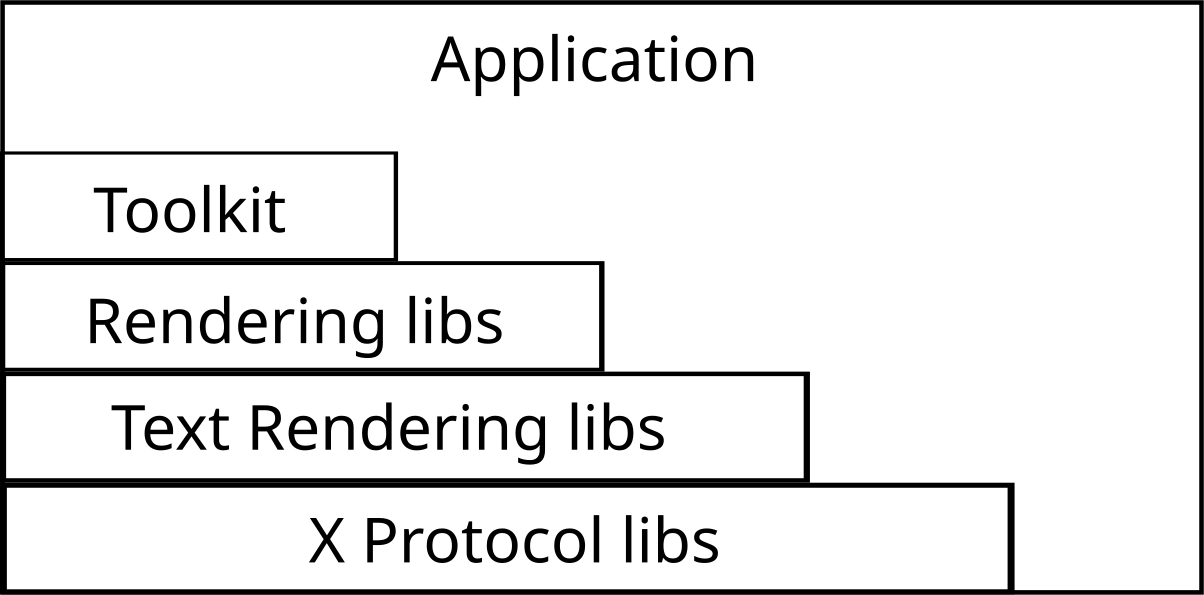
\includegraphics[scale=0.40]{x-3-1.png}
	\caption{X程序}
	\label{img-1.3.1-1}
\end{figure}

大多数X应用程序都需要渲染一些东西。X社区拥有强大的库支持,可以在大多数环境中高效、方便地绘图。这些库处理针对特定视频硬件、输出格式等的优化。对于2D图形,Cairo库目前被应用程序直接使用,也被工具包用于呈现需求。对于3D图形,OpenGL API是行业标准,由Mesa库在免费软件栈中实现。

正确的文本处理比大多数开发人员意识到的要棘手,特别是当他们只暴露于7位ASCII文本时。处理Unicode字符,为不同的语言加载适当的字体,弄清楚如何在具有复杂规则的语言中放置字符以连接字符或覆盖变音符号,甚至只是弄清楚字符是按从左到右还是从右到左的顺序显示:这些都是现有库(如Pango和HarfBuzz)解决的问题。工具包使用这些库来处理它们提供的小部件中的文本布局,Cairo使用它们来处理它呈现的画布中的文本,应用程序使用它们来处理它们需要直接放在屏幕上的任何文本。

在所有这些库的下面是X的Xft扩展。Xft提供在屏幕上实际显示文本符号,使用fontconfig为每个符号找到合适的字体,并使用FreeType将每个符号呈现为图像,Xft可以将其发送到X服务器以供显示。

与X服务器的实际通信由两组库之一处理——Xlib或XCB。每个库族都提供了对实际X协议请求的编程访问,对客户端隐藏了X11协议连接和编码/解码的细节。Xlib和XCB在本书的Xlib和XCB章节中有更详细的介绍。

虽然理论上可以使用纯系统调用编写X客户机,自己生成所有的X协议消息编码和解码,但这通常会浪费大量的时间,并且是bug的来源。也可以只使用X11库编写X客户端,并自己生成绘制菜单、按钮和文本的所有代码,但这也浪费了大量时间;要获得支持国际化、可访问性、桌面集成、输入处理和工具包提供的许多其他特性所需的全部功能,需要程序员多年的努力。

\subsection{构建X客户端代码}

X.Org以及上面提到的许多开源工具包和库,已经对pkg-config系统的使用进行了标准化,以确定在构建使用这些库的软件时需要使用的编译器和链接器标志集。

\noindent 例如,要找到链接libxcb和libxcb-util库所需的标志,你可以运行:

\begin{lstlisting}[language=C]
pkg-config --libs xcb xcb-util -lxcb-util -lxcb
\end{lstlisting}

您不应该简单地将结果复制到构建脚本中。相反,在构建时运行pkg-config:结果可能因平台、安装位置(不同的“-I”或“-L”标志来找到正确的路径)或需求变化时的版本而异。

\noindent 如果您的软件是使用GNU autoconf系统构建的,那么pkg-config提供了一个简单的宏,您可以使用它在配置中查找构建所需的标志。ac脚本。你也可以指定给定库的最低要求版本,如下例所示:

\begin{lstlisting}
PKG_CHECK_MODULES(XCBLIBS, [xcb >= 1.6] xcb-icccm xcb-shape)
\end{lstlisting}

如果找到了所有必需的库,并且有足够的版本和它们在pkg-config文件中指定的任何必需的依赖项,那么autoconf将在生成的名为XCBLIBS\_CFLAGS和XCBLIBS\_LIBS的Makefiles中提供变量。这些变量将提供需要传递给构建的编译和链接阶段的标志。

\subsection{X库}

下面的列表是由X.Org维护的提供C语言API的X库。如上所述,这些API提供了较低级别的功能,在其之上构建了来自其他提供商的较高级库。其他语言(如Python、Perl和Tcl)的语言绑定层也可以从各种来源获得。

在X协议栈的核心有两代库——较新的XCB和较旧的Xlib。本指南中的Xlib和XCB章节解释了它们之间的区别,并描述了两个系列之间的互操作性。

几乎所有这些库的文档都以Unix手册页和DocBook/XML参考文档的形式包含在库本身中。对于那些有DocBook文档的人,从这些文档生成的HTML、PDF和纯文本格式文档已经在\url{http://www.x.org/releases/current/doc/}上发布。

\subsubsection{XCB系列协议和实用程序库}

新一代的X协议编码和解码库是建立在XCB核心之上的,编码和解码函数是根据协议的XML描述自动生成的。libxcb提供了连接管理功能和核心X协议的处理,并为每个X扩展提供了额外的库:

\begin{lstlisting}
libxcb-composite    libxcb-res        
libxcb-damage       libxcb-screensaver 
libxcb-dpms         libxcb-shape            libxcb-xinerama
libxcb-dri2         libxcb-shm              libxcb-xinput
libxcb-glx          libxcb-sync         	libxcb-xprint
libxcb-randr        libxcb-xevie            libxcb-xtest
libxcb-record       libxcb-xf86dri      	libxcb-xv
libxcb-render       libxcb-xfixes       	libxcb-xvmc
\end{lstlisting}

不幸的是,由于XKB协议的复杂性,目前XCB库还不能支持所有扩展,libxcb-xkb仍在开发中。两个扩展,BigRequests和XC-MISC,是处理其他请求的基础;因此,这些扩展直接内置于libxcb中,而不是通过单独的库提供。

还有一些建立在XCB协议库之上的实用程序库,以提供常见的高级功能。这些库仍在开发中,它们的API在不同版本之间仍有一些变化,可能会破坏兼容性。

\begin{itemize}
	\item libxcb-icccm和libxcb-ewmh:这两个库提供了获取和设置ICCCM和EWMH标准中指定的属性的函数,用于与窗口管理器和桌面环境进行交互。(请参阅“概念”一章中的“属性”部分,了解更多关于这些的详细信息。)
	\item libxcb-image:这个库在X服务器之间移动图像(客户端像素图)。在Xlib中,XImage和XShmImage提供了类似的功能。
	\item libxcb-render-util:这个库为使用Render扩展绘制图像和文本提供了方便的函数。
	\item libxcb-util:这个库是一个util函数和定义的大杂烩,无法适应其他库。该库包括标准原子常量、原子缓存、事件解码和显示结构操作。
\end{itemize}

\subsubsection{xlib系列协议和使用程序库}

老一代的X协议处理程序构建在libX11之上,这是一个俗称为Xlib的库。除了协议处理之外,libX11还包括大量实用程序函数。Xlib提供对国际输入法和ICCCM属性处理的支持。它还提供了其他功能(如颜色管理)的遗留版本,现在通常在更高级别的库中提供;现代库提供了与工具包和应用程序更好的集成。与XCB家族一样,许多扩展都有自己的基于xlib的库来处理对该扩展的请求。但是,一组常见的旧扩展被分组到单个libext库中。

\noindent 扩展库:

\begin{center}
	\tablefirsthead{
		\hline
		\multicolumn{1}{|l}{库} &
		\multicolumn{1}{|l|}{说明} \\
		\hline
	}
\begin{supertabular}{|l|l|}
	libXcomposite & 窗口管理器扩展\\
	libXdamage & damage 扩展\\
	libXevie & XEvIE 扩展\\
	libXfixes & X-Fixes 扩展\\
	libXfontcache & X-TrueType 字体缓存扩展\\
	libXi & Xinput 扩展\\
	libXinerama & Xinerama 扩展\\
	libXp & Xprint 扩展\\
	libXrandr & X 屏幕大小调整、旋转扩展\\
	libXrender & render 扩展\\
	libXres & x 资源扩展\\
	libXss & MIT-SCREEN-SAVER 扩展\\
	libXTrap & X trap 扩展\\
	libXtst & XTEST扩展,Record扩展\\
	libXv & Xvideo扩展\\
	libXvMC & Xvideo运动补偿扩展\\
	libXxf86dga & XFree86直接图形访问扩展\\
	libXxf86misc & XFree86-Misc 扩展\\
	libXxf86vm & XFree86 视频模式扩展\\
	libdmx & Distributed Multihead X extension\\
	\hline
\end{supertabular}
\end{center}

\noindent libXext涵盖的扩展:

\begin{itemize}
	\item DBE:双缓冲扩展
	\item DPMS:显示电源管理信令
	\item MIT-MISC:X11R3 Bug兼容模式[已过时]
	\item AppGroup:应用程序分组[已过时]
	\item EVI:扩展视觉信息
	\item Generic Event:X通用事件扩展
	\item LBX:低带宽X[过时]
	\item MultiBuf:多重缓冲扩展[已废弃]
	\item SECURITY:X安全模型扩展
	\item SHAPE:非矩形窗口扩展
	\item MIT-SHM:共享内存图像/像素图扩展
	\item SYNC:X同步扩展
	\item TOG-CUP:色图利用协议扩展[已废弃]
	\item XTestExt1:X11输入合成扩展[已废弃]
\end{itemize}

这些扩展中有相当一部分不再常用,或者不再受X服务器的支持。但是,由于libXext将它们捆绑到同一个库中,因此在不破坏与现有程序的向后兼容性的情况下,很难删除它们。

\subsubsection{X内部工具包和传统工具包}

X.Org最初开发了X工具包内部函数(libXt),为多个工具包提供通用功能。libXt允许通过公共X资源格式、标准化事件循环和其他底层功能进行配置。libXt被用于许多早期的工具包,包括X.Org的样本Athena Widgets工具包(libXaw)、Sun的OpenLook工具包(libXol)和开放软件基金会的Motif工具包(libXm)。然而,现代工具包大多避开了libXt。这些工具包使用其他通用层(例如,用于事件循环的glib)和它们自己的工具包特定于桌面的库代码的某种组合。因此,维护libXt主要是为了供遗留应用程序使用。

Athena Widgets工具包是许多X.Org示例应用程序以及来自其他来源的一些应用程序使用的工具包。原始版本(libXaw)具有非常简单的2-D外观,而增强的版本(libXaw3d)更新了外观,具有更多的3-D感觉。这两个版本都没有积极开发。与底层libXt一样,Athena Widgets主要是为现有应用程序维护的。不鼓励使用Athena Widgets编写新的应用程序。该工具包缺乏现代应用程序正确操作所需的许多功能。例如,国际化支持很少,对屏幕阅读器或为有身体残疾的用户提供的替代输入设备等可访问性技术的支持也很少。在手机或平板电脑等非传统计算设备上使用Athena Widgets也会很尴尬。

\begin{note}
libXt和Athena库都是建立在Xlib协议处理库家族之上的。
\end{note}

\subsubsection{相关协议的库}

虽然X11协议及其扩展是X窗口系统的核心,但它们并不是X中使用的唯一协议,并且为需要在这些协议上操作的软件提供了额外的库。

\begin{itemize}
	\item libFS处理X字体服务协议的编码和解码,允许X服务器或其他程序从远程XFS字体服务器检索字体。这纯粹是遗留功能,不应该在现代客户机或服务器配置中使用。
	\item libICE支持使用客户端间交换协议在多个客户端之间进行通信。
	\item libSM涵盖了构建在libICE之上的X会话管理协议。libSM为桌面环境提供了一种机制,可以在停止X会话之前保存正在运行的客户机的状态,并在下次登录时恢复该状态。、
	\item libXdmcp为X显示管理器控制协议提供编码和解码。XDMCP提供了一个资源贫乏的本地X服务器(通常是X终端),能够对远程计算机上的客户机进行身份验证。
\end{itemize}

\subsubsection{实用工具库}

X.Org提供了一些实用程序库,方便地封装了多个客户机所需的函数。其中许多都基于Xlib协议库堆栈。

\begin{itemize}

\item libXau操作xauth、X服务器和显示管理器使用的.xauthority文件来存储共享的秘密数据,例如用于验证试图连接到X服务器的X客户机的MIT-MAGIC-COOKIEs。libXau由Xlib和XCB共同使用。
\item libXcursor处理由Render和XFixes扩展提供的alpha混合游标和动画游标,包括用于从磁盘存储和读取它们的文件格式。libXau由Xlib和XCB共同使用。(这个——po8)
\item libXfont是遗留核心协议字体呈现机制的实现。libXfont被X服务器和XFS字体服务器用来加载和呈现各种格式的字体。其中一些格式的呈现代码内置于库中。其他格式则传递给FreeType库进行栅格化。一些X.Org字体实用程序使用libXfont来管理字体文件和元数据文件,如fonts.dir。普通客户端不会直接链接到libXfont,而是通过X协议请求访问该功能。现代客户端完全避免使用X核心字体,而是依赖于fontconfig / libXft或利用这些工具的库。因此,libXfont严格代表遗留功能。
\item libfontenc处理用于跨字符编码(如ISO-8859和Unicode)映射字体的编码表。与libXfont一样,libfontenc是X.Org核心字体基础架构软件使用的遗留软件,而不是普通客户端使用的软件。
\item libXft是一个客户端直接使用的字体库。它与fontconfig合作查找字体,与FreeType合作渲染字体,并与libXrender或libX11合作将渲染文本绘制到屏幕上或像素图中。一些客户机直接使用libXft,但大多数客户机使用诸如pango之类的高级库或应用程序工具包提供的API。这些API处理文本塑造和布局规则,以确定复杂语言中字形的适当位置和连接。
\item libXmu和libXmuu是X.Org示例客户端使用的各种实用程序的集合。libXmuu包含基于核心libX11库构建的实用程序。libXmu依赖于Athena Widgets工具包,导入libXaw和libXt。
\item libXpm支持XPM XPixMap图像文件格式。XPM以可移植的ASCII文本格式表示图像数据。这在遗留的X应用程序中尤其重要,因为遗留的X应用程序倾向于将XBM或XPM映像直接编译到C代码中。现代应用程序使用外部库或工具包功能来访问映像文件。
\item libxtrans是传输层(套接字、管道等)的共享代码实现,用于X窗口系统中的许多协议实现(如libX11、libICE、libFS、xfs和X服务器)的通信。它实际上不像其他库那样是一个共享库,而是内置于每个库或程序中的共享C代码。XCB库栈在libxcb中有自己的连接管理代码,不使用xtrans。实际上,XCB取代了现代Xlib中libxtrans的几个实例之一。
\end{itemize}

\subsection{xlib和xcb}

关于Xlib和XCB,最常见的两个问题可能是“它们是什么?”和“它们有什么区别?”

如果所有编程语言都要处理X客户端与X服务端之间通信的协议内容是没必要且复杂的。因此,如果有库为X工具包和应用程序处理这些任务,并提供与编程语言和环境相适应的API来连接到X服务器,那么编写X工具包和应用程序就容易得多。

X客户端库的底层是Xlib和XCB,这两个库(实际上是库集)提供了与X服务器通信的API。Xlib和XCB具有不同的设计目标,并且是在X窗口系统演进的不同阶段开发的。

大多数应用程序开发人员应该谨慎地调用Xlib和XCB。更高级别的工具包提供了更高效的编程模型,并支持现代应用程序所期望的特性,包括支持复杂的国际化输入和输出、可访问性以及与桌面环境的集成。但是,有时应用程序会发现自己需要调用原始的底层X11库来进行工具包不支持的操作。应用程序可能需要调用工具箱编程模型当前版本中未包含的X扩展API。没有被工具包API包装的绘图也很常见。

原始的c语言X11 API是libX11,通常称为“Xlib”。它被设计成看起来像一个传统的库API,隐藏了调用导致对服务器的协议请求的事实。不需要X服务器响应的调用在缓冲区中排队,作为一批请求发送到服务器。那些需要响应的请求会刷新所有缓存的请求,然后阻塞,直到接收到响应。

Xlib的同步和异步行为混合会导致一些问题。Xlib的行为经常让新程序员感到困惑。调用有时似乎有效,而其他调用无效,因为不清楚哪些调用隐式刷新缓冲区。许多调用的异步特性使得调试问题变得困难。当报告错误时,堆栈跟踪显示接收和处理错误时正在进行的调用,通常在导致错误的调用之后进行许多调用。最后,Xlib的同步调用会导致可避免的往返延迟。这种延迟对应用程序性能有显著影响;特别是,启动时间通常会大大增加。

经过多年使用Xlib的经验,并从它和其他协议接口库中学习,为X11定义C语言绑定进行了第二次尝试:“X11 C绑定”层XCB。XCB在其设计中明确了协议的客户机-服务器特性。客户端负责决定何时刷新请求缓冲区,何时读取结果以及何时等待服务器响应。


\noindent 例如,要查找窗口属性,Xlib代码是一个函数调用:

\begin{lstlisting}[language=C]
XGetWindowProperty(dpy, win, atom, 0, 0, False, AnyPropertyType, &type_ret, &format_ret, &num_ret, &bytes_after, &prop_ret);
\end{lstlisting}

\noindent Xlib生成对X服务器的请求,以检索属性并将其附加到请求缓冲区。由于这是一个需要响应的请求,所以Xlib随后会刷新缓冲区,将内容发送到X服务器。接下来,Xlib等待,直到X服务器处理属性检索请求之前的所有请求,然后发送属性检索应答。然后Xlib将应答返回给客户机。

Xlib还提供了包装属性请求的便利函数。这些便利函数检索特定的属性,知道每个属性的详细信息以及如何请求和解码它。示例包括XGetWMName和XGetWMHints。其中一些函数可以在Xlib外部编写,但许多函数以重要的方式使用Xlib内部组件,因此是不可分割的。

另一方面,XCB以一种“显而易见”的机制方式提供了直接从协议描述生成的函数。XCB函数直接映射到协议,使用单独的函数将请求放入传出缓冲区,并稍后异步地从X服务器读取结果。以上代码的XCB版本为:
\begin{lstlisting}[language=C]
prop_cookie = xcb_get_property (dpy, False, win, atom, XCB_GET_PROPERTY_TYPE_ANY, 0, 0);
prop_reply = xcb_get_property_reply (dpy, prop_cookie, NULL);
\end{lstlisting}

\noindent XCB的强大之处在于,它允许在这两个步骤之间放置尽可能多的代码。程序员决定何时等待数据,而不是在发出请求时被迫等待请求返回的数据。

\subsubsection{示例:将xwininfo从Xlib转换为XCB}

xwininfo程序是一个命令行实用程序,用于在X服务器上打印有关windows的信息。通过命令行选项,它可以提前知道从服务器请求每个窗口信息所需的大部分数据。因此,xwininfo可以一次发出所有请求,然后等待结果的到来。当使用-tree选项遍历窗口树时,xwininfo可以一次请求当前窗口的所有子窗口的数据,甚至可以进一步批处理。在单个CPU服务器上的本地连接上,这意味着X客户机和服务器之间的上下文切换更少。在多核/CPU服务器上,X服务器可以在一个核心上处理请求,而客户机在另一个核心上处理响应,从而提高了性能。在远程连接上,可以将请求分组到更接近连接的MTU大小的数据包中,而不是在发出需要响应的请求时发送缓冲区中的任何请求。

xwininfo的1.1版本由Alan Coopersmith从Xlib转换为XCB。我们用GNOME桌面会话和几个客户端对它进行了测试。Xwininfo以“Xwininfo -root -all”的方式运行:这将在窗口层次结构的根处启动Xwininfo,并要求它遍历树,沿途请求每个窗口可用的所有信息。在这个示例会话中,它找到了114个窗口。(在X中,窗口只是一个用于绘制输出和接收事件的容器。X窗口通常是“用户窗口”周围的区域或边界)。当在四核Intel Nehalem CPU上本地运行时,两个版本都运行得非常快(0.05秒或更少),以至于时间上的差异太小,无法精确测量。为了测量远程性能,使用“ssh -X”将X11连接从加利福尼亚隧道连接到中国的一台计算机,并从那里返回到加利福尼亚的工作站,这引入了大量的延迟。在这种设置下,两者之间的差异是巨大的:
\begin{lstlisting}
Xlib: 0.03u 0.02s 8:19.12 0.0% 
xcb: 0.00u 0.00s 0:45.26 0.0% 
\end{lstlisting}

\noindent 当然,xwininfo在一些方面是一个不寻常的X应用程序:

\begin{itemize}
	\item Xwininfo尽可能快地运行请求,然后退出,而不是等待用户输入(除非您使用单击窗口选择该窗口的模式,然后它像正常一样运行)。一旦启动并运行,大多数X应用程序将大部分时间用于等待用户输入,因此通过减少与X服务器通信所花费的时间,总体运行时不会减少太多。但是,应用程序启动通常由往返时间主导,因此正确使用XCB可以减少运行在高延迟(甚至中等延迟)连接上的X应用程序的巨大启动时间。
	
	\item Xwininfo只使用核心协议和形状扩展。它不使用大多数现代应用程序使用的更复杂的扩展,如Render或Xinput。Xinput、XKB和GLX的问题特别大,因为它们还没有在XCB发行版中得到完全支持,尽管已经通过一些谷歌夏季代码项目进行了支持。
	
	\item xwininfo足够小,因此可以一次彻底修改使用XCB。大多数应用程序都比这个大得多。XCB主要针对新代码和工具包:它是专门为与现有Xlib应用程序进行互操作而设计的。对Xlib和XCB的调用可以混合使用,因此可以根据需要对Xlib应用程序进行部分转换或增量转换。
	
	\item xwininfo只使用原始Xlib,没有任何工具包。因此,它不必担心工具包使用哪个X库。
	
	\item xwininfo只使用几个Xlib帮助函数。这使得它可以更直接地映射到XCB。例如,依赖于Xlib的输入法框架、组合键处理或字符集转换的应用程序将更难移植。幸运的是,无论如何,现代工具包在工具包层处理了大部分这些功能。
\end{itemize}

xwininfo确实依赖于Xlib函数来从其他字符集转换窗口名称属性——XCB版本目前只适用于UTF-8和Latin-1窗口名称。由于大多数现代工具包使用UTF-8,因此可能没人会注意到这一点。具有本地化窗口名称的旧应用程序将失败,但很少有这样的应用程序在使用。

\subsubsection{混合Xlib和XCB调用}

如上所述,XCB提供了一种从Xlib到XCB的增量转换方法。可以使用libX11打开显示,并将它返回的display指针传递给现有代码、工具包和库。要调用XCB函数,可以将Display指针转换为相同连接的xcb\_connection\_t指针。这样就可以从同一个应用程序调用Xlib和XCB。

Xlib和XCB的兼容性是通过将libX11重新构建为libxcb之上的层来实现的。Xlib和XCB共享相同的X服务器连接并来回传递对它的控制。该选项是在libX11 1.2中引入的,自2010年libX11 1.4发布以来一直存在(不再是可选的)。

\subsubsection{示例:将xdpyinfo扩展查询转换为XCB}

xdpyinfo是标准X窗口系统工具集中的另一个命令行工具。与xwininfo一样,xdpyinfo打印大量关于X服务器的信息。Xdpyinfo调用许多扩展,其中很少有调用阻塞等待来自服务器的响应。但是,如果添加"-queryExt"选项,xdpyinfo将调用XQueryExtension来打印当前运行的服务器中分配给该扩展的请求、事件和错误id。这些id是动态分配的,并且根据给定服务器构建/配置中启用的扩展集而变化。因此,在调试引用扩展id的X错误报告时,扩展id列表是非常重要的信息。当报告来自自定义错误处理程序(如gtk工具包中的错误处理程序)的X错误消息时,特别需要使用“xdpyinfo -queryExt”:此类错误处理程序通常会忽略默认Xlib错误处理程序中找到的扩展信息,因此阅读错误报告的人将无法识别遇到错误的扩展。

Xlib调用XQueryExtension每次接受一个扩展名,向X服务器发送请求以获取该扩展的id代码,然后等待响应,以便将这些id返回给调用者。在用作此转换的测试系统的Xorg 1.7服务器上,有30个活动的X扩展,也就是发送到X服务器的30个小数据包,xdpyinfo客户机在poll()中阻塞等待响应的时间是30倍,X服务器在再次阻塞自己的select()循环之前执行客户机处理和请求调度代码的时间是30倍。

\begin{note}
注意:XListExtensions可用于获取可用扩展的列表,这些扩展可通过XQueryExtension调用。
\end{note}

对xdpyinfo的一个简单补丁将XQueryExtension调用的循环替换为两个循环。第一个循环为每个扩展调用xcb\_query\_extension。发出整个批处理查询后,第二个循环xcb\_query\_extension\_reply开始收集批处理回复。使用"truss -c"收集系统调用计数显示了xdpyinfo客户端进行的系统调用数量的预期减少:

\begin{center}
	\tablefirsthead{
		\hline
		\multicolumn{1}{|l}{系统调用} &
		\multicolumn{1}{|l|}{xlib} &
		\multicolumn{1}{|l|}{xcb}\\
		\hline
	}
	\begin{supertabular}{|l|l|l|}
		writev & 40 & 11\\
		poll & 80 & 22\\
		recv & 117 & 29\\
		total & 237 & 62\\
		\hline
	\end{supertabular}
\end{center}

\noindent 在一个TCP连接上,切换到XCB来处理这个事务既减少了数据包的数量,也减少了(由于TCP包头开销)总的数据量:
\begin{center}
	\tablefirsthead{
		\hline
		\multicolumn{1}{|l}{} &
		\multicolumn{1}{|l|}{xlib} &
		\multicolumn{1}{|l|}{xcb}\\
		\hline
	}
	\begin{supertabular}{|l|l|l|}
		TCP packets & 93 & 35\\
		TCP bytes & 11554 & 7726\\
		\hline
	\end{supertabular}
\end{center}

对于大多数应用程序来说,这种类型的更改比大规模转换为XCB要可行得多。找到应用程序正在等待来自服务器的数据的热点,并转换这些热点。在应用程序启动代码中,当应用程序收集关于X服务器和会话的信息时,几乎总是有机会。将这些调用转换为更有效的XCB调用集可以获得主要的性能优势。X开发人员早期的工作减少了许多应用程序的延迟,方法是将对XInternAtom的重复调用转换为一个调用,通过XInternAtom一次获取多个原子。XCB允许对这一原则进行推广。

\subsubsection{扩展库}

X11协议的每个新扩展都会增加客户机可以向X服务器发出的请求。为了允许客户端软件利用这些请求,大多数扩展提供了构建在Xlib或XCB之上的API。这些API使用库的连接编组将它们的请求包含在发送到X服务器的流中。

在早期的X11版本中,许多较小和更常用的扩展被分组到一个公共库libXext中。您会发现其中有几个目前仍在使用,例如MIT-SHM共享内存扩展、用于非矩形窗口的SHAPE扩展和用于事件同步的SYNC扩展。但是,libXext还包括一些API,用于当前Xorg服务器版本中不再出现的扩展,例如App-Group和Low-Bandwidth X (LBX),以及许多应用程序从不使用的扩展,例如用于显示电源管理的DPMS。由于这些扩展API不能在不破坏任何可能使用它们的现有应用程序的情况下从libext中删除,因此代码被卡在那里。

因此,新的Xlib扩展API不再添加到libext中。相反,为每个扩展创建一个利用libX11的新库。每个扩展都有一个库,可以更容易地开发该扩展的API,弃用过时的扩展,并仅将其链接到实际需要它的客户端。几乎所有现代扩展都有自己的Xlib API库——libXrender用于RENDER扩展,libXcomposite用于COMPOSITE扩展,等等。有一些扩展是协议交互的核心,它们直接在libX11本身中得到支持,比如BigRequests、XC-MISC和XKB。

当XCB将自己的API风格加入其中时,它遵循了较新的风格,并为每个扩展创建了一个以“libxcb”为前缀的库——libxcb-composite、libxcb-render等。由于XCB可以根据扩展协议的XML描述自动为扩展生成API代码,因此只需将扩展描述添加到XCB -proto包中并重新构建即可创建新的扩展API。不幸的是,一些较旧的扩展具有复杂的协议,不容易用XML语法描述。扩展语法和代码生成器以处理这些问题的工作正在进行中。XKB和GLX协议是当前面临的挑战。

\subsubsection{API文档}

要使用Xlib或XCB编写代码,您需要了解库API的详细信息。Xlib包括大多数函数的手册页,提供了很好的API参考。libext包含了一些扩展API的手册页,但不是全部。在各个基于xlib的扩展库中,手册页的覆盖率甚至更加参差不齐。

还有一个更完整的Xlib API指南,以及许多扩展API的规范,参见X.Org在线文档: \url{http://www.x.org/releases/current/doc/}

对于没有xlib风格API文档的扩展,调用通常是到上述链接文档集中提供的协议规范的简单映射。

对于XCB,文档更加依赖于协议规范。生成的API是对X协议的精确映射;它尽可能直接地将C调用数据转换为X协议编码的数据包。XCB API中的连接管理和其他功能记录在\url{http://xcb.freedesktop.org/XcbApi/}。为方便开发人员,正在向XCB添加支持,以便从XML协议描述生成Unix风格的参考手册页。

还有一个XCB教程,“使用XCB库进行基本图形编程”,网址是\url{http://www.x.org/releases/current/doc/libxcb/tutorial/index.html}。

\subsection{使用扩展}

正如在客户端和服务器之间的通信一章中所描述的,X窗口系统通过X11协议的扩展机制随着时间的推移而发展,该机制允许为客户端和服务器之间的通信定义新的协议请求、事件和错误。

希望使用扩展的客户端必须首先检查服务器是否支持该扩展,如果支持,则检查服务器支持哪个版本的扩展。一些扩展提供了一种简单的版本协商机制,其中客户端向服务器发送客户端理解的协议版本,服务器响应它在该范围内可以支持的最佳版本。如果不执行此版本检查握手,许多扩展将无法正常工作,因为客户端库或服务器中的关键数据结构将不会初始化,并且具有多个版本的扩展可能使用错误的版本进行通信,从而导致两端的解析错误。

\subsubsection{示例:使用来自基于xcb的客户机的扩展}

这个例子来自X.Org的xwininfo客户端,一个简单的客户端,检索屏幕上的窗口信息并打印出来。如果服务器支持SHAPE扩展,则可以打印非矩形窗口的形状信息,例如xeyes的圆形眼球窗口。

\noindent 在配置文件中。xwininfo声明它需要xcb库来构建形状扩展,没有xcb库就无法构建。它还需要xcb库本身的至少1.6版本。

\begin{lstlisting}
# Obtain compiler/linker options for xwininfo dependencies
PKG_CHECK_MODULES(XWININFO, [xcb >= 1.6] xcb-shape)
\end{lstlisting}

\noindent 一些客户端在构建时将扩展设置为可选的,允许构建器选择忽略对它们的支持,并使用\lstinline|#ifdef|语句等机制来隔离对它们的调用。本指南不包括这样的例子。

然后xwininfo程序代码初始化扩展并在使用它之前检查版本。shape扩展在其生命周期中有两个版本,1.0和1.1。1.1版本在1.0版本的基础上添加了一些简单的功能,这些功能不会破坏现有的功能或协议,也不会破坏使用它的客户端。

由于形状窗口的使用是与这个单一函数隔离的,如果不支持扩展,它可以简单地返回,否则它可以继续使用xcb-shape库提供的函数来封装shape扩展协议请求和应答。

\begin{lstlisting}
#include <xcb/shape.h>
[...]
static void Display_Window_Shape (xcb_window_t window)
{
	xcb_query_extension_reply_t *shape_query;
	xcb_shape_query_extents_cookie_t extents_cookie;
	xcb_shape_query_extents_reply_t *extents;
	
	shape_query = xcb_get_extension_data (dpy, &xcb_shape_id);
	if (!shape_query->present)
	return;
	
	extents_cookie = xcb_shape_query_extents (dpy, window);
	extents = xcb_shape_query_extents_reply (dpy, extents_cookie, &err);
[...]
\end{lstlisting}

\subsubsection{示例:使用来自基于xlib的客户机的扩展}

这个例子来自X.Org的xdpyinfo客户端,这是一个简单的客户端,用于检索和打印关于X服务器和显示的信息。它打印当前扩展的列表,如果通过-ext标志传递某些扩展名,则打印有关给定扩展的更多信息。它可以做到这一点的扩展之一是Xinerama扩展,它可以获取有关实际显示单个逻辑屏幕部分的监视器数量以及每个监视器显示屏幕的哪个部分的信息。

在配置文件中。xdpyinfo为构建器提供了一个命令行标志来启用或禁用对xinerama的构建支持,如果启用,则通过pkg-config检查libXinerama所需的头文件和库:

\begin{lstlisting}
AC_ARG_WITH(xinerama, AS_HELP_STRING([--without-xinerama],[Disable xinerama support.]),
[USE_XINERAMA="$withval"], [USE_XINERAMA="yes"])
if test "x$USE_XINERAMA" != "xno" ; then
	PKG_CHECK_MODULES(DPY_XINERAMA, xinerama)
else
	echo "without xinerama"
fi
\end{lstlisting}

在代码中,Xinerama支持是\lstinline|#ifdef|的,所以它只在配置脚本找到扩展库时才编译。代码为此使用“PANORAMIX”,因为这是Xinerama最初建议的名称,并且当扩展名称最终确定时,代码没有得到更新。根据需要,客户端所做的第一件事是查询扩展的存在及其版本,然后如果它在兼容版本中可用,则继续对扩展本身进行调用。

\begin{lstlisting}
#ifdef PANORAMIX
#include <X11/extensions/Xinerama.h>
#endif
#ifdef PANORAMIX
static int print_xinerama_info(Display *dpy, const char *extname)
{
	int majorrev, minorrev;
	if (!XineramaQueryVersion (dpy, &majorrev, &minorrev)) return 0;
	print_standard_extension_info(dpy, extname, majorrev, minorrev);
	if (!XineramaIsActive(dpy)) {
		printf("  Xinerama is inactive.\n");
	} else {
		int i, count = 0;
		XineramaScreenInfo *xineramaScreens = 
		XineramaQueryScreens(dpy, &count);
		[...]
\end{lstlisting}

\subsection{X键盘扩展}

X键盘扩展(XKB)负责一些键盘行为,更重要的是,它定义了客户端看到的键盘布局。

用户看到的XKB与服务器看到的XKB有很大的不同,本章将解释接口之间的差异以及它们如何生成可被客户端使用的键盘布局。

关于键盘处理最重要的一点是,传递的值几乎总是键码——一个与上下文无关的数字,表示键盘上的键。密钥码必须在8到255之间,并且相同的物理密钥每次都应生成相同的密钥码。除此之外,键码没有语义意义,它们只是作为各种查找表的索引。

\subsubsection{RMLVO和Kccgst}

键盘配置的核心是两个接口:“规则(Rules)、模型(Model)、布局(Layout)、变量(Variant)、选项(Options)”(RMLVO)和“键码(Keycode) Compat Geometry Symbols Types”(Kccgst)。理解这两个接口之间的共生关系是理解键盘配置的关键。

\subsubsection{RMLVO}

RMLVO键盘配置通常通过各种用户接口公开。用户通常希望将键盘布局设置为本地化符号集合的组合,例如“us”或“de”布局,以及该集合的可能变体,例如“dvorak”而不是默认的“qwerty”。

可以使用其他选项进行进一步配置,这些选项通常启用或更改单个密钥或操作。常用的选项是启用服务器操作,例如关闭(终止)服务器或重新分配键码,例如将Caps Lock更改为Compose键码。

这些选项、布局和变体的定义在规则文件中定义。现在只有两个规则文件重要:evdev和base,前者是大多数当代GNU/Linux系统的规则文件,后者是其他系统的规则文件。规则文件是简单的查找表,形式为“对于这个布局,加载这个符号描述”。好奇的读者可以在大多数发行版的/usr/share/X11/xkb/rules中找到它们。规则附带一个xml文件,为每个值提供人类可读的描述。这些xml文件由gui使用。

最后,模型是键实际存在于特定键盘模型上的表示。由于Linux内核的抽象,模型的权重比以前要小,大多数键盘只使用“evdev”模型。

一旦用户指定了所需的RMLVO组合,这些描述将被转换为Kccgst描述,然后加载到服务器中。RMLVO查找和翻译所需的所有文件都由xkeyboard-config模块提供,通常位于/usr/share/x11/xkb中

有关RMLVO的更多信息请访问:\url{http://who-t.blogspot.com.au/2008/09/rmlvo-keyboard-configuration.html}

\subsubsection{Kccgst}

RMLVO是用户友好的,但不完整,它没有定义“us”布局的实际含义。这是Kccgst文件的工作,以及相互匹配的规则。

当用户指定布局“us”时,该模型将与该模型的“Keycodes”部分、该模型的“Geometry”部分和“us”“Symbols”部分相匹配。“Types”和“Compat”在很大程度上是默认设置,稍后将对它们进行描述。

“Geometry”最容易解释:它描述了每个键的物理位置和尺寸。除了允许客户端显示键盘的外观之外,它没有其他用途。这也是Kccgst中唯一不是强制性的部分。“Geometry”很大程度上基于模型,因此对于那些没有自己的模型和几何形状的键盘,使用抽象的、更通用的几何形状。

“Keycodes”部分简单地为键及其数字代码分配符号名称。键码按行分组,qwerty布局上“Q”键的符号名称是AD01-d行第一个键。其他符号名称是FK03(第三个功能键),LCTL(左控制键)等。这些符号名称仅在Kccgst描述中有用,并用作查找。

Symbols部分实际描述了键的作用。它将键码的符号名称与该键所代表的符号进行匹配。在qwerty布局中,“Q”键看起来是这样的:

键{type= "ALPHABETIC",符号[Group1]=[q, q]};

在azerty布局中,相同的键看起来像这样:key {type= "ALPHABETIC", symbols[Group1]= [a, a]};

\begin{note}
注意,符号名是相同的,因为物理键生成相同的键码,而不管布局如何。
\end{note}

这个键的例子显示了一个有2个“级别”的键。Types部分定义了键的各种类型以及按下修饰符时的行为。在“符号”部分为每个键分配了一个类型。上面显示的字母类型默认情况下生成第一层的符号,如果Shift或CapsLock修饰符在逻辑上是无效的,则生成第二层的符号。其他类型可以使用其他修饰符,如AltGr, Ctrl+Alt等。但在所有情况下,修饰符组合只是指该键的特定级别。

Symbols部分定义了哪些键映射到哪些修饰符。下面的示例显示左shift键和右shift键都映射到shift修饰符,从而触发字母类型中的第二级。

\begin{lstlisting}
	modifier_map Shift { <LFSH> };
	modifier_map Shift { <RTSH> };
\end{lstlisting}

Compat部分定义键组合时发生的操作。这些动作包括终止服务器、移动指针、在布局之间切换等等。

最后注意:在上面的示例中,这些符号是为Group1定义的。每个键最多可以有4组,其中一组在该键盘上的任何时间都处于活动状态。这允许同时加载多个布局,并在布局之间快速切换。

\subsubsection{从RMLVO到Kccgst的转换}

RMLVO在很大程度上只是一个用户特定的界面,服务器处理Kccgst。这个过程分为两个步骤:首先,将RMLVO转换为简单的Kccgst描述,这主要是通过匹配RMLVO来完成的,而不需要查看实际的部分。然后,将简单的Kccgst转换为完整的描述。然后将该描述加载到(或由)服务器。

\noindent 一个简单的Kccgst描述可能是这样的:

\begin{lstlisting}
xkb_keymap {
	xkb_keycodes  { include "evdev+aliases(qwerty)" };
	xkb_types     { include "complete"      };
	xkb_compat    { include "complete"      };
	xkb_symbols   { include "pc+us+inet(evdev)+compose(caps)+terminate(ctrl_alt_bksp)"     };
	xkb_geometry  { include "pc(pc104)"     };
};
\end{lstlisting}

从简单Kccgst到完整描述的转换由xkbcomp进程处理,xkbcomp是一个词法解析器,它读取所有文件并组装最终描述。xkbcomp可以生成文本描述或称为“XKM”的二进制格式,该格式与X服务器内部使用的C结构非常接近。

在服务器启动时,服务器为每个键盘派生xkbcomp,并加载xkbcomp生成的xkm文件。目前正在努力将xkbcomp的核心转移到libxkbcommon库中,以避免分叉。

\subsubsection{Key处理}

一旦设置好键盘布局,键处理的过程就相对简单了。键码由驱动程序提交。服务器检查键码并在适用的情况下更改修饰符状态。它还检查要对该键执行的所有操作。一旦完成,键码将作为键事件发送到客户端。

然后,客户端将键码和修饰符状态与先前从服务器获得的键盘布局进行匹配,并在响应中执行一些操作。服务器提供修饰符状态和键码,但这取决于客户端希望如何处理该键。它可能完全忽略修饰语,甚至将符号更改为完全不同的东西。

\subsection{字体}

如“X客户端生态系统”一章所述,X有两个字体系统,原始的核心X11字体系统和较新的Xft字体系统。

X11的核心字体系统直接来源于1987年X11R1附带的字体系统,该系统只能使用单色位图字体。多年来,它或多或少被强制用于处理可缩放字体和旋转字形。

Xft从一开始就被设计为对可伸缩字体提供良好的支持,并且是高效的。与核心字体系统不同,它支持抗锯齿和亚像素光栅化等功能。也许更重要的是,它使应用程序能够完全控制字形的呈现方式,从而实现精细的排版和所见即所的显示。最后,它允许应用程序使用没有安装在系统范围内的字体来显示带有嵌入字体的文档。

Xft与核心字体系统不兼容:使用Xft需要对工具包进行相当广泛的更改,在某些情况下还需要对应用程序进行更改。在X.Org继续维护核心字体系统的同时,鼓励客户端软件作者尽快切换到Xft。

有关使用和配置X字体系统的更多信息,请参见\url{http://www.x.org/releases/X11R7.7/doc/xorg-docs/fonts/fonts.html}。该文档还包括计算机字体的一般背景资料和指向其他参考站点的指针,首先阅读这些部分可能有助于理解以下部分。

\subsubsection{核心字体系统}

在最初的X11字体机制中,如果X客户端希望以12点大小的Times New Roman字体呈现某些文本,则需要首先调用XLoadFont()来使用XLFD字体名称“-adobe-times-medium-r-normal——12-120-75-75-p-64-iso8859-1”打开字体。服务器打开该字体(使用libXfont中的例程)并返回与打开字体相关的XID,然后应用程序将其存储在相关的GC中,以供以后的绘图操作。如果没有找到该字体,客户机可以使用XListFonts()请求可用字体列表——因为XLFD报告每个点大小、样式变体(粗体、斜体、罗马体、精简体等)和支持的编码(iso8859-*用于较旧的文本编码,iso10646-1用于Unicode)都有一个单独的字体名称,大多数X服务器将返回一个包含数千个字体条目的列表,这可能需要很长时间才能通过低带宽远程连接发送。

在绘制文本之前,许多客户端首先需要确定绘制时字符串的大小(例如,调整按钮的大小或对文本区域进行换行)。为此,客户机调用带有字符串和字体信息的XTextExtents(), X服务器以简单的并排顺序排列文本,并返回结果边界框和大小信息。如果需要另一种布局,例如泰语或阿拉伯语等语言的复杂布局,则客户端必须自己进行布局。为了将文本拟合到一个区域中,这可能涉及多次往返,尝试字符串的不同子集,从而增加了文本绘制操作的延迟。

实际上,绘制文本是通过XDrawString()或XDrawText()调用完成的,它们再次重做并排布局。每个XDrawString()调用只能绘制一条文本的水平线,尽管沿着基线的字符可以单独旋转。文本是单色绘制的,没有抗锯齿,使用从GC传递给调用的前景和背景颜色以及字体选择。每次调用只能绘制单一字体的字符,文本来自单一编码,因此将iso8859-1中的英文文本与big5-1中的中文字符混合需要多次调用。XDrawText()允许在一次调用中传递多个字符串,每个字符串都有不同的字体属性集。

每个调用文本字符串都有多种变体,这取决于文本字符串是如何编码的,例如,对于XDrawString()实际上有:

\begin{center}
	\begin{supertabular}{|l|l|l|}
		\hline
		XDrawString & Single byte text\\
		XDrawString16 & Double byte text\\
		XmbDrawString & Multibyte text\\
		XwcDrawString & Wide character text\\
		Xutf8DrawString & UTF-8 multibyte text\\
		\hline
	\end{supertabular}
\end{center}

如果你不知道所有这些不同的文本编码类型是什么,你可以了解更多关于各种编码文本的方法:

\begin{itemize}
	\item \url{http://www.joelonsoftware.com/articles/Unicode.html}
	\item \url{https://en.wikipedia.org/wiki/Category:Character_encoding}
	\item \url{http://shop.oreilly.com/product/9780596102425.do}
\end{itemize}

\subsection{客户端字体}

一个新的字体系统在21世纪初被设计和实现,它与传统的核心字体系统并存,允许旧客户端和新客户端一起运行。新的字体系统将大部分工作转移到客户端,减少了往返次数并降低了绘制字体所需的延迟。它还增加了对复杂文本布局的更好支持,利用渲染扩展中的alpha混合支持为文本渲染提供抗锯齿和LCD优化,并允许客户端使用文档或应用程序中可用的字体,而不需要首先将它们安装在X服务器中,或者必须使用X字体服务(xfs)来提供对它们的远程访问。

X.Org为这个字体系统提供的API是libXft,但它通常位于文本处理和字体渲染技术堆栈的中间。客户机使用它们的工具包提供的文本接口,或者使用一般的高级呈现API(如Cairo)。它们使用Pango或Qt布局引擎(可能与HarfBuzz引擎一起)来确定如何将字形放在彼此相邻的位置以形成单词,并在必要时重塑它们以适应其上下文。这些API依次使用FontConfig库为所需的每个字符集或字形找到可用的字体,并使用FreeType库从各种格式的字体中光栅化图像,例如OpenType, TrueType, PCF或Type1。然后libXft库将图像文本发送到X服务器,使用Render扩展字形缓存来避免重新发送具有统一外观的常见字符,并且Render扩展将文本与底层图像数据组合在一起,通过与边缘像素的alpha通道混合来实现抗锯齿效果。

该系统允许客户端在本地计算布局,而无需往返于服务器;沿着他们选择的任何基线绘制文本,而不仅仅是一个水平基线;并允许在客户端中插入对各种不同文本处理模型的支持,这取决于他们的需要,而无需修改X服务器或在可能具有特权的X服务器进程中运行代码。FontConfig提供了一种更可用和人类可读的字体命名方案,使用上面提到的12点Times New Roman的长XLFD名称而不是简单的“Times New Roman-12”。

新的字体呈现模型在现代应用程序和工具包(如Gtk+和Qt)中被广泛采用,而维护原始的X11核心字体子系统是为了向后兼容尚未更新的遗留X11应用程序。

\subsection{X客户端与X服务端交互的调试}

调试X客户端应用程序带来了额外的挑战,因为问题通常不仅仅出现在运行的程序中,还涉及到与X服务器的交互,并且可能需要监视X服务器正在做什么,或者监视X客户端与服务器之间的通信。有几个工具可用于此操作。

\subsubsection{事件上报}

有时,问题就像试图找出X服务器为某个键或按钮按下或其他输入发送的事件一样简单。X.Org样例应用程序中包含的xev程序提供了一种简单的方法来实现这一点—只需运行xev\footnote{archlinux 系统需要安装 xorg-xev 包},将焦点放在其窗口上,并导致事件发生,然后它将打印出详细信息。例如,按下并释放键盘上的“e”键会从xev生成以下输出:

\begin{lstlisting}
KeyPress event, serial 115, synthetic NO, window 0x4a00001,
root 0x15a, subw 0x0, time 170495410, (948,265), root:(966,365),
state 0x0, keycode 26 (keysym 0x65, e), same_screen YES,
XLookupString gives 1 bytes: (65) "e"
XmbLookupString gives 1 bytes: (65) "e"
XFilterEvent returns: False

KeyRelease event, serial 115, synthetic NO, window 0x4a00001,
root 0x15a, subw 0x0, time 170495531, (948,265), root:(966,365),
state 0x0, keycode 26 (keysym 0x65, e), same_screen YES,
XLookupString gives 1 bytes: (65) "e"
XFilterEvent returns: False
\end{lstlisting}

\subsubsection{X资源扩展}

客户机可以向X服务器发出几种类型的请求,以代表客户机在X服务器中分配内存,例如创建窗口或像素图。当用户抱怨X服务器内存增长时,通常是由于客户机分配了这些内存而没有清理它们。虽然X服务器将在客户端退出时释放与客户端关联的大部分资源,但这并不能阻止像web浏览器这样的长寿命客户端在客户端运行时增加内存。

为了解决这个问题,创建了X-resource扩展,以允许客户端了解为X服务器中的每个客户端执行的分配。有几个客户端可以查询这些信息。在GNOME中,通过在Preferences中显示的信息字段中启用X server memory列,Performance Monitor应用程序可以显示每个客户机的X服务器内存使用总量。

xrestop程序显示每个客户机的更详细信息,按资源类型分解使用情况,该程序可从\url{http://www.freedesktop.org/wiki/Software/xrestop}获得。

\subsubsection{协议监控}

有几个程序可以监视X协议连接并显示解码的数据包,以显示客户机发出的请求以及服务器在响应中发送的应答、错误和事件。这些包括:
\begin{itemize}
	\item xscope \url{http://www.x.org/releases/individual/app/}
	\item x11vis
	\item xmon
	\item xtrace
	\item wireshark
\end{itemize}

\noindent 其中前四种是X协议代理服务器——在启动客户机之前,必须首先启动代理并将其配置为连接到当前X服务器的新xserver。例如,常见的配置是Xorg服务器以:0运行,xscope以:1运行。然后需要将客户机设置为连接到xscope服务器,该服务器依次打印它在真实服务器和客户机之间来回传递的通信。

使用xtrace需要注意的一点是,您可能需要使用-n选项来绕过身份验证问题。例如:

\begin{lstlisting}
jcomeau@aspire:~$ xtrace -o /tmp/skype.xtrace skype
No display name to create specified, trying :9
Error parsing xauth list data: less than three things in a line!
\end{lstlisting}

但是使用 -n:

\begin{lstlisting}
jcomeau@aspire:~$ xtrace -n -o /tmp/skype.xtrace skype
No display name to create specified, trying :9
Got connection from unknown(local)
...
[starts skype successfully]
\end{lstlisting}

Wireshark是一款网络协议监视器。与代理风格的监视器不同,它可以在客户机生命周期中的任何时间启动,但它只监视通过tcp套接字的连接,而不是本地连接。它实际上是一个通用的网络协议分析器,支持数百种协议,X11只是其中之一。

\subsubsection{系统级跟踪}

Solaris、MacOS和FreeBSD上的DTrace工具,以及Linux上的SystemTap工具,提供了跨程序跟踪操作的能力,并在客户端和服务器之间将它们关联起来。详细文档可以查看:\url{http://www.x.org/releases/current/doc/}

\chapter{Xlib——X的C语言接口}


\section{xlib简介}

X的前10个版本的设计和实现主要是由三个人完成的:麻省理工学院计算机科学实验室的罗伯特·舍弗勒、数字设备公司的吉姆·盖提斯和麻省理工学院的罗恩·纽曼,他们都是麻省理工学院雅典娜项目的成员。然而,X的第11个版本则是许多地方和组织共同努力的成果。

X窗口系统是麻省理工学院设计的一个网络透明窗口系统。X显示服务器运行在具有单色或彩色位图显示硬件的计算机上。服务器将用户输入分发给位于同一台机器上或网络中其他地方的各种客户机程序,并接受它们的输出请求。Xlib是一个C子例程库,应用程序(客户端)使用它通过流连接与窗口系统进行交互。尽管客户机通常运行在与其通信的X服务器所在的同一台机器上,但情况并非如此。

Xlib−C语言X接口是X窗口系统协议的低级C语言接口的参考指南。它既不是教程,也不是X窗口系统编程的用户指南。相反,它提供了库中每个函数的详细描述以及相关背景信息的讨论。Xlib−C语言X界面假定对图形窗口系统和C编程语言有基本的了解。其他高级抽象(例如,由X工具包提供的抽象)构建在Xlib库之上。有关这些高级库的进一步信息,请参阅相应的工具包文档。X窗口系统协议(Window System Protocol)\footnote{\url{https://www.x.org/releases/current/doc/}}提供了关于X的行为的权威词汇。尽管这里出现了额外的信息,但协议文档是主导文档。

\subsection{X窗口系统概述}

本书中使用的一些术语是X所独有的,而其他窗口系统通用的其他术语在X中具有不同的含义。您可能会发现参考位于本书末尾的术语表会有所帮助。

X窗口系统支持一个或多个包含重叠窗口或子窗口的屏幕。屏幕是一个物理显示器和硬件,可以是彩色、灰度或单色的。每个显示器或工作站可以有多个屏幕。单个X服务器可以为任意数量的屏幕提供显示服务。单个用户使用一个键盘和一个指针(通常是鼠标)的一组屏幕称为显示器。

X服务器中的所有窗口都按照严格的层次结构进行安排。在每个层次结构的顶部是一个根窗口,它覆盖了每个显示屏幕。每个根窗口部分或全部被子窗口覆盖。除根窗口外,所有窗口都有父窗口。通常每个应用程序至少有一个窗口。子窗口可能会有自己的子窗口。通过这种方式,应用程序可以在每个屏幕上创建任意深度的树。X为窗口提供图形、文本和光栅操作。

子窗口可以比父窗口大。也就是说,子窗口的部分或全部可以扩展到父窗口的边界之外,但是窗口的所有输出都被其父窗口剪切。如果一个窗口的几个子窗口有重叠的位置,则认为其中一个子窗口位于其他子窗口之上或高于其他子窗口,从而使它们变得模糊。输出到其他窗口覆盖的区域将被窗口系统抑制,除非该窗口具有后备存储。如果一个窗口被第二个窗口遮挡,第二个窗口只遮挡第二个窗口的祖先,同时也是第一个窗口的祖先。

窗口的边框宽度为0或更多像素,可以是任何图案(像素图)或您喜欢的纯色。一个窗口通常(但不总是)有一个背景图案,当被揭开时,它将被窗口系统重新绘制。子窗口掩盖了父窗口,父窗口中的图形操作通常由子窗口剪切。

每个窗口和像素图都有自己的坐标系统。坐标系的X轴为水平轴,Y轴为垂直轴,原点[0,0]位于左上角。坐标是积分的,以像素为单位,并与像素中心重合。对于窗口,原点在内部左上角的边界内。

X不保证保留窗口的内容。当一个窗口的部分或全部被隐藏,然后再回到屏幕上,它的内容可能会丢失。然后,服务器向客户端程序发送一个Expose事件,通知它需要重新绘制部分或全部窗口。程序必须准备好在需要时重新生成窗口的内容。

X还提供图形对象的屏幕外存储,称为pixmaps。单平面(深度为1)像素图有时被称为位图。像素图可以在大多数图形函数中与窗口互换使用,并在各种图形操作中用于定义模式或块。窗口和像素图一起被称为可绘制图。

Xlib中的大多数函数只是将请求添加到输出缓冲区。这些请求稍后在X服务器上异步执行。返回存储在服务器中的信息值的函数在接收到显式回复或发生错误之前不会返回(也就是说,它们会阻塞)。您可以提供一个错误处理程序,它将在报告错误时被调用。

如果客户端不希望请求异步执行,它可以在请求之后调用XSync,该调用将阻塞,直到所有先前缓冲的异步事件都被发送并执行。作为一个重要的副作用,Xlib中的输出缓冲区总是在调用任何从服务器返回值或等待输入的函数时被刷新。

许多Xlib函数将返回一个整数资源ID,它允许您引用存储在X服务器上的对象。这些类型可以是Window、Font、Pixmap、Colormap、Cursor和GContext,如文件<X11/X.h>中定义的。这些资源由请求创建,并在请求或连接关闭时销毁(或释放)。这些资源中的大多数都可能在应用程序之间共享,事实上,窗口是由窗口管理器程序显式地操纵的。字体和游标在多个屏幕之间自动共享。字体根据需要加载和卸载,并由多个客户端共享。字体通常缓存在服务器中。Xlib不支持在应用程序之间共享图形上下文。

客户端程序被告知事件。事件可能是请求的副作用(例如,重新堆叠窗口生成Expose事件),也可能是完全异步的(例如,来自键盘)。客户端程序要求获得事件通知。由于其他应用程序可以向您的应用程序发送事件,因此程序必须准备好处理(或忽略)所有类型的事件。

输入事件(例如,按下键或指针移动)从服务器异步到达,并排队,直到显式调用(例如,XNextEvent或XWindowEvent)请求它们。此外,一些库函数(例如XRaiseWindow)会生成Expose和ConfigureRequest事件。这些事件也是异步到达的,但是客户机可能希望在调用一个函数之后通过调用XSync显式地等待它们,该函数会导致服务器生成事件。

\subsection{错误}

一些函数返回Status(一个表示错误信息的整数)。如果函数失败,则返回0。如果函数返回状态为0,则表示它没有更新返回参数。由于C语言不提供多个返回值,因此许多函数必须通过写入客户端传递的存储来返回结果。默认情况下,错误由标准库函数或您提供的函数处理。如果字符串不存在,返回指向字符串指针的函数返回NULL指针。

X服务器在检测到协议错误时候就会报告错误信息。如果一个给定的请求可以生成多个错误,服务器可以报告其中的任何一个。

由于Xlib通常不会立即将请求传输到服务器(也就是说,它会缓冲请求),因此报告错误的时间可能比实际发生的时间晚得多。然而,出于调试目的,Xlib提供了一种强制同步行为的机制(参见11.8.1节)。当启用同步时,错误会在生成时报告。

当Xlib检测到错误时,它调用程序可以提供的错误处理程序。如果不提供错误处理程序,则打印错误并终止程序。

\subsection{标准头文件}

\begin{itemize}
	\item <X11/Xlib.h>:这是Xlib的主要头文件。大多数Xlib符号都是通过包含这个文件来声明的。该文件还包含预处理器符号XlibSpecificationRelease。此符号在本标准中定义为6。(Xlib的第5版是第一个有这个符号的版本。)
	\item <X11/X.h>:该文件声明了应用程序将使用的X协议的类型和常量。它从<X11/Xlib.h>自动包含,因此应用程序代码不需要直接引用该文件。
	\item <X11/Xcms.h>:这个文件包含了第6章中描述的许多颜色管理工具的符号。所有以“Xcms”为前缀的函数、类型和符号,以及颜色转换上下文宏,都在这个文件中声明。在包含此文件之前必须包含<X11/Xlib.h>。
	\item <X11/Xutil.h>:该文件声明了用于客户端间通信和应用程序实用程序的各种函数、类型和符号,这些将在第14章和第16章中描述。在包含此文件之前必须包含<X11/Xlib.h>。
	\item <X11/Xresource.h>:该文件声明了资源管理器设施的所有函数、类型和符号,这些将在第15章中描述。在包含此文件之前必须包含<X11/Xlib.h>。
	\item <X11/Xatom.h>:该文件声明了所有预定义的原子,这些原子是前缀为“XA\_”的符号。
	\item <X11/cursorfont.h>:该文件声明了标准游标字体的游标符号,它们列在附录b中。所有的游标符号都有前缀“XC\_”。
	\item <X11/keysymdef.h>:该文件声明了所有标准KeySym值,这些值是前缀为“XK\_”的符号。键盘系统按组排列,预处理器符号控制每组的包含。必须在包含文件之前定义预处理器符号以获得相关值。预处理器符号是xk\_miscellaneous, XK\_XKB\_KEYS, XK\_3270, XK\_LATIN1, XK\_LATIN2, XK\_LATIN3, XK\_LATIN4, XK\_KATAKANA, XK\_ARABIC, XK\_CYRILLIC, XK\_GREEK, XK\_TECHNICAL, XK\_SPECIAL, XK\_PUBLISHING, XK\_APL, XK\_HEBREW, XK\_THAI和XK\_KOREAN。
	\item <X11/keysym.h>:这个文件定义了预处理器符号xk\_miscellaneous, XK\_XKB\_KEYS, XK\_LATIN1, XK\_LATIN2, XK\_LATIN3, XK\_LATIN4和XK\_GREEK,然后包括<X11/keysymdefh>。
	\item <X11/Xlibint.h>:该文件声明了用于扩展的所有函数、类型和符号,这些在附录c中有描述。该文件自动包含<X11/Xlib.h>。
	\item <X11/Xproto.h>:该文件声明了基本X协议的类型和符号,以便在实现扩展时使用。它从<X11/xlibin.h>自动包含,因此应用程序和扩展代码不需要直接引用该文件。
	\item <X11/Xprotostr.h>:该文件声明了基本X协议的类型和符号,以便在实现扩展时使用。它从<X11/xproto1.h>自动包含,因此应用程序和扩展代码不需要直接引用该文件。
	\item <X11/X10.h>:该文件声明了用于X10兼容性函数的所有函数、类型和符号,这些在附录D中有描述。
\end{itemize}

\subsection{常用值和类型}

\noindent 以下符号由Xlib定义,并在整个手册中使用:
\begin{itemize}
	\item Xlib定义Bool类型和布尔值True和False。
	\item None是通用的空资源ID或原子。
	\item 类型XID用于通用资源id。
	\item 类型XPointer定义为char*,并用作指向数据的泛型不透明指针。
\end{itemize}

\subsection{Xlib中的命名和参数约定}

Xlib在函数的命名和语法方面遵循许多约定。假设您记住了函数需要的信息,这些约定旨在使函数的语法更加可预测。

\noindent 主要的命名约定有:

\begin{itemize}
	\item 为了将X符号与其他符号区分开来,库对外部符号使用混合大小写。按照现有约定,它为变量保留小写字母,为用户宏保留全部大写字母。
	\item 所有Xlib函数都以大写X开头。
	\item 所有函数名和符号的开头都大写。
	\item 所有用户可见的数据结构都以大写X开头。更一般地说,用户可以解引用的任何内容都以大写X开头。
	\item 宏和其他符号不以大写x开头。为了区别于所有用户符号,宏中的每个单词都大写。
	\item 数据结构中的所有元素或变量都是小写的。必要时,复合词用下划线(\_)构成。
	\item 当使用display参数时,它总是在参数列表的第一个。
	\item 所有使用的资源对象都出现在参数列表的开头,紧跟在display参数之后。
	\item 当图形上下文与另一种类型的资源(最常见的是可绘制的资源)一起出现时,图形上下文出现在参数列表中,位于其他资源之后。可抽取资源的排名高于所有其他资源。
	\item 在参数列表中,源参数总是位于目标参数之前。
	\item 在参数列表中,x参数总是位于y参数之前。
	\item 在参数列表中,宽度参数总是位于高度参数之前。
	\item 当x、y、width和height参数一起使用时,x和y参数总是在width和height参数之前。
	\item 当掩码与结构体同时出现时,掩码总是位于参数列表中指向该结构体的指针之前。
\end{itemize}

\subsection{编程注意事项}

\noindent 主要的编程考虑是:

\begin{itemize}
	\item X中的坐标和大小实际上是16位的量。这个决定是为了最小化给定性能级别所需的带宽。坐标通常在接口中声明为int。大于16位的值将被静默截断。尺寸(宽度和高度)被声明为无符号数量。
	\item 键盘是不同制造商工作站之间最大的变量。如果你希望你的程序是可移植的,你应该在这里特别保守。
	\item 许多显示系统的屏幕外内存有限。如果可以的话,应该尽量减少像素图和后备存储的使用。
	\item 用户应该能够控制自己的屏幕空间。因此,您应该编写应用程序来响应窗口管理,而不是假定控制整个屏幕。但是,在顶层窗口内执行的操作取决于应用程序。有关更多信息,请参阅第14章和客户端间通信约定手册。
\end{itemize}

\subsection{字符集和编码}

\noindent 一些Xlib函数引用了特定的字符集和字符编码。以下是最常见的:

\subsubsection{x可移植字符集(X Portable Character Set)}

97个字符的基本集合,假定存在于Xlib支持的所有语言环境中。该字符集包含以下字符:

\begin{lstlisting}
a..z
A..Z
0..9
!"#$\%&'()*+,-./:;<=>?@[\\]^_`{|}~
<space>, <tab>, <newline>
\end{lstlisting}

该字符集是ISO8859-1图形字符集的左/下半部分加上空格、制表符和换行符。它也是7位ASCII的图形字符集加上相同的三个控制字符。这些字符在主机上的实际编码取决于系统。

\subsubsection{主机可移植字符编码}

主机上X可移植字符集的编码。编码本身不是由这个标准定义的,但是在主机上Xlib支持的所有语言环境中,编码必须是相同的。如果一个字符串被称为主机可移植字符编码,那么它只包含来自主机编码的X可移植字符集的字符。

\subsubsection{Latin-1}

由ISO8859-1标准定义的编码字符集。

\subsubsection{Latin可移植字符编码}

使用Latin-1码点加上ASCII控制字符对X可移植字符集进行编码。如果一个字符串被称为Latin Portable Character Encoding,那么它只包含来自X Portable Character Set的字符,而不是Latin-1的所有字符。

\subsubsection{STRING编码}

Latin-1,加上制表符和换行符。

\subsubsection{POSIX可移植文件名字符集}

65个字符的集合,可用于在posix兼容的主机上命名文件,在所有语言环境中都能正确处理。集合为:


\begin{lstlisting}
a..z
A..Z
0..9
._-
\end{lstlisting}

\subsubsection{格式规范}

\noindent Xlib−C语言X接口使用以下约定:

\begin{itemize}

\item 全局符号以这种特殊字体打印。这些可以是函数名、包含文件中定义的符号或结构名。在声明和定义时,函数参数以斜体打印。在后面的解释性文字中,它们通常是用普通字体打印的。
\item 每个函数都是通过一般性讨论来介绍的,以区别于其他函数。函数声明本身紧随其后,并对每个参数进行了具体解释。虽然没有使用ANSI C函数原型语法,但Xlib头文件通常使用ANSI C环境中的函数原型来声明函数。如果需要对函数进行一般性讨论,则在参数之后进行。在适用的情况下,说明的最后一段列出了函数可能生成的Xlib错误码。有关Xlib错误码的完整讨论,请参见第11.8.2节。
\item 为了消除您传递的参数和函数返回给您的参数之间的任何歧义,您传递的所有参数的解释都以单词specify开头,或者在有多个参数的情况下,以单词specify开头。返回给您的所有参数的解释都以单词returns开头,或者在有多个参数的情况下,以单词return开头。您可以传递和返回的所有参数的解释都以单词指定和返回开始。
\item 任何指向用于返回值的结构体的指针都由\_return后缀作为其名称的一部分指定。传递给这些函数的所有其他指针仅用于读取。一些参数使用指向结构体的指针,这些结构体同时用于输入和输出,并使用\_in\_out后缀表示。
\end{itemize}

\section{显示(Display)相关函数}

\noindent 在您的程序可以使用显示器之前,您必须建立到X服务器的连接。一旦建立了连接,就可以使用本章讨论的Xlib宏和函数来返回有关显示的信息。本章讨论以下几点:

\begin{itemize}
	\item 打开(连接到)显示器
	\item 获取有关显示、图像格式或屏幕的信息
	\item 生成一个NoOperation协议请求
	\item 释放客户端创建的数据
	\item 关闭(断开)显示器
	\item 使用X服务器关闭连接操作
	\item 使用带有线程的Xlib
	\item 使用内部连接
\end{itemize}

\subsection{打开显示器}

要打开到控制显示的X服务器的连接,请使用XOpenDisplay。

\begin{lstlisting}[language=C]
	Display* XOpenDisplay(char* display_name);
\end{lstlisting}

\begin{note}
	display\_name: 指定硬件显示名称,该名称确定要使用的显示和通信域。在符合posix的系统上,如果display\_name为NULL,则默认为DISPLAY环境变量的值。
\end{note}

XOpenDisplay函数返回一个Display结构,该结构用作到X服务器的连接,并且包含关于该X服务器的所有信息。XOpenDisplay通过TCP或DECnet通信协议,或通过某些本地进程间通信协议,将应用程序连接到X服务器。如果协议指定为“tcp”、“inet”或“inet6”,或者没有指定协议,主机名是主机名,主机名和显示号之间用一个冒号分隔,XOpenDisplay使用tcp流连接。(如果指定的协议为“inet”,则使用TCP over IPv4。如果指定协议为inet6,则使用TCP over IPv6。否则,实现将决定使用哪个IP版本。)如果没有指定主机名和协议,Xlib将使用它认为最快的传输方式。如果主机名是主机名,用双冒号(::)分隔主机名和显示号,XOpenDisplay使用DECnet进行连接。单个X服务器可以同时支持任何或所有这些传输机制。特定的Xlib实现可以支持更多这样的传输机制。

如果成功,XOpenDisplay返回一个指向Display结构的指针,该结构在<X11/Xlib.h>中定义。如果XOpenDisplay不成功,它返回NULL。在成功调用XOpenDisplay之后,客户机可以使用显示中的所有屏幕。display\_name参数中指定的屏幕编号由DefaultScreen宏(或XDefaultScreen函数)返回。只能通过使用信息宏或函数来访问Display和Screen结构的元素。有关使用宏和函数从Display结构中获取信息的信息,请参见2.2.1节。

\subsection{获取有关显示、图像格式或屏幕的信息}

Xlib库提供了许多有用的宏和相应的函数,它们从Display结构返回数据。这些宏用于C编程,它们对应的函数等价于其他语言绑定。本节讨论:

\begin{itemize}
	\item 显示宏
	\item 图像格式函数和宏
	\item 屏幕信息宏
\end{itemize}

Display结构的所有其他成员(即没有为其定义宏的成员)都是Xlib私有的,不能使用。应用程序绝对不能直接修改或检查Display结构的这些私有成员。下一节中的XDisplayWidth、XDisplayHeight、XDisplayCells、XDisplayPlanes、XDisplayWidthMM和XDisplayHeightMM函数命名不当。这些函数应该命名为Screenwhatever和XScreenwhatever,而不是Displaywhatever或XDisplaywhatever。对于由此造成的混乱,我们深表歉意。

\subsubsection{Display Macros}

应用程序不应该直接修改Display和Screen结构的任何部分。这些成员应该被认为是只读的,尽管它们可能会由于对显示的其他操作而改变。下面列出了C语言的宏,它们对应的用于其他语言绑定的等价函数,以及它们都可以返回的数据。

\begin{lstlisting}[language=C]
unsigned long XAllPlanes(void);
unsigned long XBlackPixel(Display *display, int screen_number);
unsigned long XWhitePixel(Display *display, int screen_number);
int XConnectionNumber(Display *display);
Colormap XDefaultColormap(Display *display, int screen_number);
int XDefaultDepth(Display *display, int screen_number);
int *XListDepths(Display *dsp, int screen_num, int* count_ret);
GC XDefaultGC(Display *display, int screen_number);
Window XDefaultRootWindow(Display *display);
Screen *XDefaultScreenOfDisplay(Display *display);
Screen *XScreenOfDisplay(Display *display, int screen_number);
int XDefaultScreen(Display *display);
Visual *XDefaultVisual(Display *display, int screen_number);
int XDisplayCells(Display *display, int screen_number);
int XDisplayPlanes(Display *display, int screen_number);
char *XDisplayString(Display *display);
long XExtendedMaxRequestSize(Display *display);
long XMaxRequestSize(Display *display);
unsigned long XLastKnownRequestProcessed(Display *display);
unsigned long XNextRequest(Display *display);
int XProtocolVersion(Display *display);
int XProtocolRevision(Display *display);
int XQLength(Display *display);
Window XRootWindow(Display *display, int screen_number);
int XScreenCount(Display *display);
char *XServerVendor(Display *display);
int XVendorRelease(Display *display);
\end{lstlisting}

\subsubsection{图像格式函数和宏}

应用程序需要以服务器要求的格式向X服务器提供数据。为了帮助简化应用程序,转换数据所需的大部分工作都由Xlib提供(参见第8.7和16.8节)。

XPixmapFormatValues结构提供了在连接建立时返回的像素图格式信息的接口。它包含:

\begin{lstlisting}[language=C]
typedef struct {
	int depth;
	int bits_per_pixel;
	int scanline_pad;
} XPixmapFormatValues;
\end{lstlisting}

\noindent 要获取给定显示的像素图格式信息,请使用XListPixmapFormats,其中 count\_return 表示:返回显示所支持的像素图格式的数目。

\begin{lstlisting}[language=C]
XPixmapFormatValues* XListPixmapFormats(
	Display* display,
	int* count_return);
\end{lstlisting}

\noindent XListPixmapFormats函数返回一个XPixmapFormatValues结构数组,这些结构描述了指定显示所支持的Z格式图像的类型。如果可用内存不足,XListPixmapFormats返回NULL。要为XPixmapFormatValues结构释放已分配的存储空间,请使用XFree。

\noindent 下面列出了C语言宏、它们对应的用于其他语言绑定的等价函数,以及它们为指定的服务器和屏幕返回的数据。这些通常被工具包和简单的应用程序使用。

\begin{lstlisting}[language=C]
int XImageByteOrder(Display *display);
\end{lstlisting}

\noindent 两者都为XY格式(位图)的每个扫描线单元或Z格式的每个像素值指定图像所需的字节顺序。宏或函数可以返回LSBFirst或MSBFirst。
\begin{lstlisting}[language=C]
int XBitmapUnit(Display *display);
\end{lstlisting}

\noindent 两者都以位为单位返回位图扫描线的大小。扫描线以该值的倍数计算。
\begin{lstlisting}[language=C]
int XBitmapBitOrder(Display *display);
\end{lstlisting}

\noindent 在每个位图单元中,屏幕上显示的位图中最左边的位要么是该单元中最不重要的位,要么是最重要的位。这个宏或函数可以返回LSBFirst或MSBFirst。
\begin{lstlisting}[language=C]
int XBitmapPad(Display *display);
\end{lstlisting}

\noindent 每个扫描线必须填充为该宏或函数返回的位的倍数。
\begin{lstlisting}[language=C]
int XDisplayHeight(Display *display, int screen_number);
\end{lstlisting}

\noindent 两者都返回一个以像素为单位描述屏幕高度的整数。
\begin{lstlisting}[language=C]
int XDisplayHeightMM(Display *display, int screen_number);
\end{lstlisting}

\noindent 以下都是返回屏幕宽度。
\begin{lstlisting}[language=C]
int XDisplayWidth(Display *display, int screen_number);
int XDisplayWidthMM(Display *display, int screen_number);
\end{lstlisting}

\subsubsection{屏幕信息宏}

\noindent 下面列出了C语言宏,它们对应的用于其他语言绑定的等价函数,以及它们都可以返回的数据。这些宏或函数都有一个指向适当屏幕结构的指针。
\begin{lstlisting}[language=C]
unsigned long XBlackPixelOfScreen(Screen *screen);
unsigned long XWhitePixelOfScreen(Screen *screen);
int XCellsOfScreen(Screen *screen);
Colormap XDefaultColormapOfScreen(Screen *screen);
int XDefaultDepthOfScreen(Screen *screen);
GC XDefaultGCOfScreen(Screen *screen);
Visual *XDefaultVisualOfScreen(Screen *screen);
int XDoesBackingStore(Screen *screen);
Bool XDoesSaveUnders(Screen *screen);
Display *XDisplayOfScreen(Screen *screen);
long XScreenNumberOfScreen(Screen *screen);
long XEventMaskOfScreen(Screen *screen);
int XWidthOfScreen(Screen *screen);
int XHeightOfScreen(Screen *screen);
int XWidthMMOfScreen(Screen *screen);
int XHeightMMOfScreen(Screen *screen);
int XMaxCmapsOfScreen(Screen *screen);
int XMinCmapsOfScreen(Screen *screen);
int XPlanesOfScreen(Screen *screen);
Window XRootWindowOfScreen(Screen *screen);
\end{lstlisting}

\subsection{生成一个 NoOperation 协议请求}

\noindent 要执行NoOperation协议请求,请使用XNoOp。XNoOp函数向X服务器发送一个NoOperation协议请求,从而执行连接。
\begin{lstlisting}[language=C]
XNoOp(Display *display);
\end{lstlisting}

\subsection{释放客户端创建的数据}

\noindent 要释放由Xlib函数创建的内存数据,请使用XFree。XFree函数是一个通用的Xlib例程,用于释放指定的数据。必须使用它来释放由Xlib分配的任何对象,除非为该对象显式指定了替代函数。NULL指针不能传递给这个函数。
\begin{lstlisting}[language=C]
XFree(void *data);
\end{lstlisting}

\subsection{关闭显示器}

\noindent 要关闭显示或断开与X服务器的连接,请使用XCloseDisplay。

\begin{lstlisting}[language=C]
XCloseDisplay(Display *display);
\end{lstlisting}

\noindent XCloseDisplay函数关闭与X服务器的连接,用于display结构中指定的显示,并销毁客户端在此显示上创建的所有窗口,资源id (Window, Font, Pixmap, Colormap, Cursor和GContext)或其他资源,除非客户端的关闭模式被更改(参见XSetCloseDownMode)。因此,不应该再引用这些窗口、资源id和其他资源,否则将生成错误。退出之前,应该显式地调用XCloseDisplay,以便在XCloseDisplay执行最后的XSync操作时报告任何挂起的错误。

\begin{note}
XCloseDisplay会生成BadGC错误。
\end{note}

\noindent Xlib提供了一个函数,允许客户端拥有的资源在客户端连接关闭后继续存在。要更改客户端的关闭模式,请使用XSetCloseDownMode。
\begin{lstlisting}[language=C]
XSetCloseDownMode(Display *display, int close_mode);
\end{lstlisting}

\noindent XSetCloseDownMode函数定义了在连接关闭时客户端资源将发生什么。连接以DestroyAll模式启动。有关close\_mode参数为RetainPermanent或RetainTemporary时客户端资源会发生什么情况的信息,请参见2.6节。

\begin{note}
XSetCloseDownMode会产生一个BadValue错误。
\end{note}

\subsection{使用X服务器连接关闭操作}

\noindent 当X服务器通过显式调用XCloseDisplay或由退出的进程关闭与客户端的连接时,X服务器执行以下自动操作:

\begin{itemize}
	\item 它否定客户端拥有的所有选择(参见XSetSelectionOwner)。
	\item 如果客户端主动抓取了指针或键盘,则执行XUngrabPointer和XUngrabKeyboard操作。
	\item 如果客户端已抓取服务器,则执行XUngrabServer。
	\item 它释放客户端所做的所有被动抓取。
	\item 它将客户端分配的所有资源(包括颜色映射项)标记为永久或临时,这取决于关闭模式是RetainPermanent还是RetainTemporary。然而,这并不能阻止其他客户端应用程序显式地销毁资源(参见XSetCloseDownMode)。
\end{itemize}

\noindent 当关闭模式为DestroyAll时,X服务器将销毁客户端的所有资源,如下所示:

\begin{itemize}
\item 它检查客户端保存集中的每个窗口,以确定它是否是客户端创建的窗口的下级(子窗口)。(保存集是被称为保存集窗口的其他客户端窗口的列表。)如果是这样,X服务器将保存集窗口重新定位到最近的祖先,这样保存集窗口就不会比客户端创建的窗口逊色。重定位使保存集窗口左上角的绝对坐标(相对于根窗口)保持不变。
\item 如果保存集窗口未被映射,它将对保存集窗口执行MapWindow请求。
\item 它会销毁客户端创建的所有窗口。
\item 它对客户端在服务器中创建的每个非窗口资源(例如,Font、Pixmap、Cursor、Colormap和GContext)执行适当的空闲请求。
\item 它释放由客户端应用程序分配的所有颜色和色图项。
\end{itemize}

当最后一个到X服务器的连接关闭时,将进行额外的处理。X服务器会经历一个没有连接和有一些连接的循环。当与X服务器的最后一个连接由于使用DestroyAll的close\_mode关闭连接而关闭时,X服务器执行以下操作:

\begin{itemize}
\item 它会重置它的状态,就好像它刚刚启动一样。X服务器首先销毁来自以RetainPermanent或RetainTemporary模式终止的客户端的所有遗留资源。
\item 它删除除预定义的原子标识符之外的所有标识符。
\item 它删除所有根窗口上的所有属性(参见4.3节)。
\item 它重置所有设备映射和属性(例如,按键、铃声音量和加速度)以及访问控制列表。
\item 它恢复标准的根磁贴和游标。
\item 它恢复默认字体路径。
\item 它将输入焦点恢复到状态PointerRoot。
\end{itemize}

\noindent 但是,如果关闭模式设置为RetainPermanent或RetainTemporary关闭连接,则X服务器不会重置。

\subsection{使用带有线程的Xlib}

\noindent 在支持的系统上,允许多个线程并发地使用Xlib。要初始化对并发线程的支持,请使用XInitThreads。

\begin{lstlisting}[language=C]
Status XInitThreads(void);
\end{lstlisting}

XInitThreads函数初始化Xlib对并发线程的支持。该函数必须是多线程程序调用的第一个Xlib函数,并且必须在进行任何其他Xlib调用之前完成。如果初始化成功,此函数返回非零状态;否则,返回0。在不支持线程的系统上,这个函数总是返回零。

只有当多个线程可能并发地使用Xlib时,才需要调用这个函数。如果对Xlib函数的所有调用都受到某种其他访问机制的保护(例如,工具箱中的互斥锁或通过显式客户机编程),则不需要Xlib线程初始化。建议单线程程序不要调用这个函数。

要跨多个Xlib调用锁定一个display,请使用XLockDisplay。XLockDisplay函数阻止所有其他线程使用指定的显示。其他试图使用该显示的线程将阻塞,直到该线程解锁该显示。嵌套调用XLockDisplay工作正确;直到XUnlockDisplay被调用的次数与XLockDisplay相同,显示才会真正被解锁。除非使用XInitThreads为线程成功初始化Xlib,否则此函数不起作用。

XUnlockDisplay函数允许其他线程再次使用指定的显示。任何在显示上被阻塞的线程都被允许继续。嵌套锁工作正确;如果一个线程多次调用XLockDisplay,那么在实际解锁显示之前,必须调用相同次数的XUnlockDisplay。除非使用XInitThreads为线程成功初始化Xlib,否则此函数不起作用。

\begin{lstlisting}[language=C]
XLockDisplay(Display *display);
XUnlockDisplay(Display *display);
\end{lstlisting}

\subsection{使用内部连接}

除了连接到X服务器之外,Xlib实现可能还需要连接到其他类型的服务器(例如,第13章中描述的输入法服务器)。使用多个显示器或将显示器与其他输入结合使用的工具包和客户端需要获得这些额外的连接以正确地阻塞,直到输入可用,并且需要在输入可用时处理该输入。在Xlib事件函数中使用单个显示和块作为输入的简单客户机不需要使用这些功能。

\noindent 要跟踪显示器的内部连接,请使用XAddConnectionWatch。

\begin{lstlisting}[language=C]
typedef void (*XConnectionWatchProc)(Display *display, XPointer client_data, int fd, Bool opening, XPointer *watch_data);
Status XAddConnectionWatch(Display *display, XConnectionWatchProc procedure, XPointer client_data);
\end{lstlisting}

XAddConnectionWatch函数注册一个过程,在Xlib每次打开或关闭指定显示的内部连接时调用该过程。传递给过程的是显示、指定的client\_data、连接的文件描述符、指示连接是打开还是关闭的布尔值,以及指向私有监视数据位置的指针。如果open为True,过程可以在watch\_data所指向的位置存储一个指向私有数据的指针;当稍后对同一连接调用该过程并且open为False时,watch\_data所指向的位置将保存相同的私有数据指针。

这个函数可以在打开显示后的任何时间调用。如果内部连接已经存在,在XAddConnectionWatch返回之前,将立即为每个内部连接调用已注册的过程。如果过程成功注册,XAddConnectionWatch返回一个非零状态;否则,返回0。

注册的过程不应该调用任何Xlib函数。如果过程直接或间接导致内部连接或监视过程的状态发生变化,则不定义结果。如果已经为线程初始化了Xlib,则调用过程时会锁定显示,并且过程对锁定显示的任何Xlib函数的调用结果都没有定义,除非执行线程使用XLockDisplay从外部锁定了显示。

\noindent 要停止跟踪显示的内部连接,请使用XRemoveConnectionWatch。XRemoveConnectionWatch函数删除先前注册的连接监视过程。client\_data必须与过程最初注册时使用的client\_data匹配。
\begin{lstlisting}[language=C]
Status XRemoveConnectionWatch(Display *display, XConnectionWatchProc procedure, XPointer client_data);
\end{lstlisting}

\noindent 要处理内部连接上的输入,请使用XProcessInternalConnection。
\begin{lstlisting}[language=C]
void XProcessInternalConnection(Display *display, int fd);
\end{lstlisting}

\noindent XProcessInternalConnection函数处理内部连接上可用的输入。只有在操作系统功能(例如select或poll)指示输入可用后,才应该为内部连接调用此函数;否则,效果没有定义。

\noindent 要获取显示器的所有当前内部连接,请使用XInternalConnectionNumbers。
\begin{lstlisting}[language=C]
Status XInternalConnectionNumbers(Display *display, int ** fd, int * count_return);
\end{lstlisting}

\noindent XInternalConnectionNumbers函数返回当前为指定显示打开的所有内部连接的文件描述符列表。当不再需要分配的列表时,使用XFree释放它。如果列表被成功分配,这个函数返回一个非零状态;否则,返回0。

\section{窗口(Window)相关函数}

\subsection{视觉类型}

在某些显示硬件上,可能以多种方式处理色彩资源。例如,您可能能够处理12位深度的屏幕,其中像素到颜色(伪色)的任意映射,或者24位深度的屏幕,其中8位像素分别用于红色,绿色和蓝色。这些处理屏幕视觉方面的不同方式被称为视觉效果。对于显示器的每个屏幕,可能有一个在屏幕不同深度处支持的有效可视类型列表。因为默认窗口和可视类型是为每个屏幕定义的,所以大多数简单的应用程序不需要处理这种复杂性。Xlib提供了返回默认根窗口、默认根窗口的默认深度和默认可视类型的宏和函数(参见第2.2.1和16.7节)。

Xlib使用不透明的Visual结构,其中包含有关可能的颜色映射的信息。可视化实用程序函数(参见第16.7节)使用XVisualInfo结构将这些信息返回给应用程序。这个结构体的成员是class、red\_mask、green\_mask、blue\_mask、bits\_per\_rgb和colormap\_size。类成员指定屏幕可能的可视类之一,可以是StaticGray、StaticColor、TrueColor、GrayScale、PseudoColor或DirectColor。

以下概念可能有助于更清楚地解释视觉类型。屏幕可以是彩色的或灰度的,可以有一个可写的或只读的颜色映射,也可以有一个颜色映射,它的索引被分解成单独的RGB块,前提是它不在灰度屏幕上。这导致了下图:

\begin{center}
	\tablefirsthead{
		\hline
		\multicolumn{1}{|l}{} &
		\multicolumn{2}{|c}{Color} &
		\multicolumn{2}{|c|}{Gray-Scale} \\
		\multicolumn{1}{|l}{} &
		\multicolumn{1}{|l}{R/O} &
		\multicolumn{1}{l|}{R/W} &
		\multicolumn{1}{l}{R/O} &
		\multicolumn{1}{l|}{R/W} \\
		\hline
	}
	\begin{supertabular}{|l|l|l|l|l|}
		Undecomposed & Static & Pseudo & Static & Gray\\
		Colormap & Color & Color & Gray & Scale\\
		Decomposed & True & Direct & & \\
		Colormap & Color & Color & & \\
		\hline
		
	\end{supertabular}
\end{center}

从概念上讲,当从显存中读取每个像素以便在屏幕上显示时,它通过索引到颜色映射来经历查找阶段。颜色映射可以在某些硬件上任意操作,在其他硬件上以有限的方式操作,而在其他硬件上则完全不能操作。视觉类型通过以下方式影响颜色图和RGB值:

\begin{itemize}
	\item 对于PseudoColor,像素值索引颜色图以生成独立的RGB值,并且RGB值可以动态更改。
	\item 灰度的处理方式与PseudoColor相同,只是驱动屏幕的原色是未定义的。因此,客户端应该始终在颜色映射中为红色、绿色和蓝色存储相同的值。
	\item 对于DirectColor,像素值被分解为单独的RGB子字段,每个子字段分别索引对应值的颜色图。RGB值可以动态更改。
	\item TrueColor的处理方式与DirectColor相同,除了颜色映射具有预定义的只读RGB值。这些RGB值依赖于服务器,但在每个主服务器中提供线性或近似线性的斜坡。
	\item StaticColor的处理方式与PseudoColor相同,只是颜色映射具有预定义的、只读的、依赖于服务器的RGB值。
	\item 处理StaticGray的方式与处理StaticColor的方式相同,只是RGB值对于任何单个像素值都是相等的,因此会产生灰色阴影。具有两项颜色映射的StaticGray可以被认为是单色的。
\end{itemize}

red\_mask, green\_mask和blue\_mask成员仅为DirectColor和TrueColor定义。每个都有一组连续的位,没有交集。bits\_per\_rgb成员指定以2为基数的红、绿、蓝不同颜色值的数量。实际的RGB值是无符号的16位数字。colormap\_size成员定义了新创建的colormap中可用的colormap条目的数量。对于DirectColor和TrueColor,这是单个像素子字段的大小。

\noindent 使用XVisualIDFromVisual从visual中获取可视ID。
\begin{lstlisting}[language=C]
VisualID XVisualIDFromVisual(Visual *visual);
\end{lstlisting}

\noindent XVisualIDFromVisual函数的作用是:返回指定可视类型的可视ID。

\subsection{窗口属性}

所有的InputOutput窗口都有一个边框宽度为零或更多像素的边框,一个可选的背景,一个事件抑制掩码(用于抑制子事件的传播),以及一个属性列表。窗口边框和背景可以是纯色或图案,称为tile。除了根目录之外的所有窗口都有一个父窗口,并被它们的父窗口剪切。如果一个窗口被堆叠在另一个窗口的顶部,为了输入的目的,它会遮蔽其他窗口。如果一个窗口有背景(几乎所有的窗口都有),为了输出的目的,它会掩盖其他窗口。输出到模糊区域的尝试不做任何事情,并且不会为模糊区域生成输入事件(例如,鼠标运动)。

\noindent Windows也有相关的属性列表

\noindent InputOutput和InputOnly窗口都有以下共同属性,这是InputOnly窗口的唯一属性:

\begin{itemize}
	\item win-gravity
	\item event-mask
	\item do-not-propagate-mask
	\item override-redirect
	\item cursor
\end{itemize}

如果为InputOnly窗口指定任何其他属性,则会导致BadMatch错误。

InputOnly窗口用于在不需要InputOutput窗口的情况下控制输入事件。InputOnly窗口是不可见的;只能用于控制诸如游标、输入事件生成和抓取之类的东西;并且不能用于任何图形请求。注意,InputOnly窗口不能将InputOutput窗口作为下级。

窗口具有可编程宽度和图案的边框以及背景图案或平铺。像素值可用于纯色。背景和边界像素图可以在创建窗口后立即销毁,如果没有进一步明确引用它们。模式可以是相对于父模式的,也可以是绝对模式的。如果ParentRelative,则使用父母的背景。

当第一次创建窗口时,它们在屏幕上不可见(不映射)。对屏幕上不可见且没有后备存储的窗口的任何输出都将被丢弃。应用程序可能希望在将窗口映射到屏幕之前创建一个窗口。当一个窗口最终映射到屏幕时(使用XMapWindow),如果没有维护后备存储,X服务器将为该窗口生成一个Expose事件。

窗口管理器可以覆盖您对顶级窗口的大小、边框宽度和位置的选择。您的程序必须准备好使用顶部窗口的实际大小和位置。除非直接响应人工命令,否则客户端应用程序不能自行调整大小。相反,您的程序应该使用给定的空间,或者如果空间太小,无法进行任何有用的工作,您的程序可能会要求用户调整窗口大小。对于窗口管理器来说,顶级窗口的边界被认为是公平的。

要设置窗口的属性,请在后续调用XCreateWindow和xchangewindowwatattributes时设置xsetwindowatattributes结构的适当成员和相应值位掩码中的OR,或者使用其他设置适当属性的方便函数之一。值掩码位和xsetwindowatattributes结构的符号是:

\begin{lstlisting}[language=C]
/* Window attribute value mask bits */
#define    CWBackPixmap                    (1L<<0)
#define    CWBackPixel                     (1L<<1)
#define    CWBorderPixmap                  (1L<<2)
#define    CWBorderPixel                   (1L<<3)
#define    CWBitGravity                    (1L<<4)
#define    CWWinGravity                    (1L<<5)
#define    CWBackingStore                  (1L<<6)
#define    CWBackingPlanes                 (1L<<7)
#define    CWBackingPixel                  (1L<<8)
#define    CWOverrideRedirect              (1L<<9)
#define    CWSaveUnder                     (1L<<10)
#define    CWEventMask                     (1L<<11)
#define    CWDontPropagate                 (1L<<12)
#define    CWColormap                      (1L<<13)
#define    CWCursor                        (1L<<14)


/* Values */
typedef struct {
	/* background, None, or ParentRelative */
	Pixmap background_pixmap;  
	
	/* background pixel */   
	unsigned long background_pixel;
	
	/* border of the window or CopyFromParent */     
	Pixmap border_pixmap;   
	
	/* border pixel value */       
	unsigned long border_pixel; 
	
	/* one of bit gravity values */    
	int bit_gravity;  
	
	/* one of the window gravity values */   
	int win_gravity;
	
	/* NotUseful, WhenMapped, Always */     
	int backing_store;     
	
	/* planes to be preserved if possible */
	unsigned long backing_planes; 
	
	/* value to use in restoring planes */    
	unsigned long backing_pixel;  
	
	/* should bits under be saved? (popups) */   
	Bool save_under;     
	
	/* set of events that should be saved */
	long event_mask;     
	
	/* set of events that should not propagate */
	long do_not_propagate_mask;  
	
	/* boolean value for override_redirect */   
	Bool override_redirect;   
	
	/* color map to be associated with window */  
	Colormap colormap;   
	
	 /* cursor to be displayed (or None) */  
	Cursor cursor;         
} XSetWindowAttributes;
\end{lstlisting}

\noindent 下面列出了每个窗口属性的默认值,并指出该属性是否适用于InputOutput和InputOnly窗口:

\begin{center}
	\tablefirsthead{
		\hline
		\multicolumn{1}{|l}{Attribute} &
		\multicolumn{1}{|l}{Default} &
		\multicolumn{1}{l|}{InputOutput} &
		\multicolumn{1}{l|}{InputOnly} \\
		\hline
	}
	\begin{supertabular}{|l|l|l|l|}
		background-pixmap & None & Yes & No \\
		background-pixel & Undefined & Yes & No \\
		border-pixmap & CopyFromParent & Yes & No \\
		border-pixel & Undefined & Yes & No \\
		bit-gravity & ForgetGravity & Yes & No \\
		win-gravity & NorthWestGravity & Yes & Yes \\
		backing-store & NotUseful & Yes & No \\
		backing-planes & All ones & Yes & No \\
		backing-pixel & zero & Yes & No \\
		save-under & False & Yes & No \\
		event-mask & empty set & Yes & Yes \\
		do-not-propagate-mask & empty set & Yes & Yes \\
		override-redirect & False & Yes & Yes \\
		colormap & CopyFromParent & Yes & No \\
		cursor & None & Yes & Yes \\
		\hline
	\end{supertabular}
\end{center}

\subsection{背景属性}

只有输入输出窗口可以有背景。您可以使用像素或像素图来设置InputOutput窗口的背景。

窗口的background-pixmap属性指定用于窗口背景的像素图。这个像素图可以是任何大小,尽管某些大小可能比其他大小快。窗口的background-pixel属性指定用于以单一颜色绘制窗口背景的像素值。

您可以将背景像素图设置为像素图、None(默认)或ParentRelative。您可以将窗口的背景像素设置为任何像素值(无默认值)。如果指定背景像素,它将覆盖默认背景像素或您可能在背景像素中设置的任何值。使用未定义大小的像素图填充背景像素作为背景。背景像素未进行距离检查;它只是被截断到适当的位数。

如果设置背景像素图,它将覆盖默认值。背景像素图和窗口必须具有相同的深度,否则会导致BadMatch错误。如果将background-pixmap设置为None,则窗口没有定义背景。如果你将背景像素图设置为ParentRelative:

\begin{itemize}
	\item 使用父窗口的背景像素图。但是,子窗口必须具有与其父窗口相同的深度,否则会导致BadMatch错误。
	\item 如果父窗口的背景像素图为None,则该窗口的背景像素图也为None。
	\item 不会生成父窗口背景像素图的副本。每次需要子窗口的背景像素图时,都会检查父窗口的背景像素图。
	\item 背景平铺原点总是与父窗口的背景平铺原点对齐。如果背景像素图不是ParentRelative,则背景贴图的原点是子窗口的原点。
\end{itemize}

设置新背景,无论是通过设置背景像素还是背景像素,都会覆盖之前的任何背景。如果没有对background-pixmap进行进一步的显式引用,则可以立即释放它(X服务器将保留一个副本以便在需要时使用)。如果稍后将其绘制到用于背景的像素图中,则会发生什么情况是未定义的,因为X实现可以自由地复制该像素图或使用相同的像素图。

当窗口的区域没有有效的内容可用,并且区域是可见的或者服务器正在维护后备存储时,服务器会自动将该区域与窗口的背景平铺,除非该窗口的背景为None。如果背景为None,则只要内容来自该窗口的父窗口或父窗口的下级窗口,则与该窗口深度相同的其他窗口的先前屏幕内容将被保留在原地。否则,暴露区域的初始内容是未定义的。然后为区域生成暴露事件,即使背景像素图为None。

\subsection{边框属性}

只有InputOutput窗口可以有边框。您可以使用像素或像素图来设置InputOutput窗口的边框。

窗口的border-pixmap属性指定用于窗口边框的像素图。窗口的border-pixel属性指定了一个未定义大小的像素图,其中填充了用于窗口边界的像素。背景像素未进行距离检查;它只是被截断到适当的位数。边框贴图的原点总是与背景贴图的原点相同。

您还可以将border-pixmap设置为任意大小的像素图(有些可能比其他像素图更快)或CopyFromParent(默认)。您可以将边框像素设置为任何像素值(无默认值)。

如果设置边框像素图,它将覆盖默认值。边界像素图和窗口必须具有相同的深度,否则会导致BadMatch错误。如果将border-pixmap设置为CopyFromParent,则复制父窗口的border-pixmap。后续对父窗口边框属性的更改不会影响子窗口。但是,子窗口必须具有与父窗口相同的深度,否则会导致BadMatch错误。

如果没有对边界像素图进行进一步的显式引用,则可以立即释放它。如果稍后绘制用于边界的像素图,则会发生什么情况是未定义的,因为X实现可以自由地复制像素图或使用相同的像素图。如果指定了边框像素,它将覆盖默认边框像素或您可能在边框像素中设置的任何值。窗口边框中的所有像素都将被设置为边框像素。设置新边框(无论是通过设置border-pixel还是通过设置border-pixmap)都会覆盖以前的任何边框。

窗口的输出总是被裁剪到窗口的内部。因此,图形操作永远不会影响窗口边框。

\subsection{Gravity属性}

窗口的位重力定义了在调整InputOutput窗口大小时应该保留窗口的哪个区域。位重力属性的默认值是ForgetGravity。窗口的窗口重力允许您定义在其父窗口大小被调整时,InputOutput或InputOnly窗口应该如何重新定位。win-gravity属性的默认值是NorthWestGravity。

如果没有更改窗口的内部宽度或高度,并且如果移动窗口或更改其边框,则窗口的内容不会丢失,而是随着窗口移动。更改窗口的内部宽度或高度会导致其内容被移动或丢失(取决于窗口的位重力),并导致子窗口被重新配置(取决于它们的win-gravity)。对于宽度和高度的变化,定义(x, y)对:

\end{sloppypar}

\backmatter
% bibliography, glossary and index would go here.

\end{document}